% ****************************************************************************************** % Dissertation template and document class for Princeton University
% Author  : Jeffrey Scott Dwoskin <jdwoskin@princeton.edu>
% Adapted from: http://www.math.princeton.edu/graduate/tex/puthesis.html
% ****************************************************************************************** %


%%% For print copies
%% set 'singlespace' option to set entire thesis to single space, and define "\printmode" to remove all hyperlinks for printed copies of the thesis. Delete all output files before changing this mode -- it will turn hyperref package on and off
%\documentclass[12pt,lot, lof, singlespace]{puthesis}
%\newcommand{\printmode}{}

%%% For the electronic copy, use doublespacing, define "\proquestmode" to use outlined links, instead of colored links. 
\documentclass[12pt]{puthesis}
\newcommand{\proquestmode}{}
% I prefer proquestmode to be off for electronic copies for normal use, since the colored links are less distracting. However when printed in black and white, the colored links are difficult to read. 

%%% For early drafts without some of the frontmatter
% Also see the "ifodd" command below to disable more frontmatter
%\documentclass[12pt]{puthesis}

%%%%%%%%%%%%%%%%%%%%%%%%%%%%%%%%%%%%%%%%%%%%%%%%%%%%%%%%%%%%%\
%%%% Author & title page info

\title{Implementing a high-performance key-value store using a trie of B+-Trees with cursors}

\submitted{June 2018}  % degree conferral date (January, April, June, September, or November)
\copyrightyear{2018}  % year in which the copyright is secured by publication of the dissertation.
\author{Oluwatosin Victor Adewale}
\adviser{Professor Andrew Appel}  %replace with the full name of your adviser
%\departmentprefix{Program in}  % defaults to "Department of", but programs need to change this.
\department{Computer Science}

%%%%%%%%%%%%%%%%%%%%%%%%%%%%%%%%%%%%%%%%%%%%%%%%%%%%%%%%%%%%%\
%%%% Tweak float placements
% From: http://mintaka.sdsu.edu/GF/bibliog/latex/floats.html "Controlling LaTeX Floats"
% and based on: http://www.tex.ac.uk/cgi-bin/texfaq2html?label=floats
% LaTeX defaults listed at: http://people.cs.uu.nl/piet/floats/node1.html

% Alter some LaTeX defaults for better treatment of figures:
    % See p.105 of "TeX Unbound" for suggested values.
    % See pp. 199-200 of Lamport's "LaTeX" book for details.
    %   General parameters, for ALL pages:
    \renewcommand{\topfraction}{0.85}	% max fraction of floats at top
    \renewcommand{\bottomfraction}{0.6}	% max fraction of floats at bottom
    %   Parameters for TEXT pages (not float pages):
    \setcounter{topnumber}{2}
    \setcounter{bottomnumber}{2}
    \setcounter{totalnumber}{4}     % 2 may work better
    \setcounter{dbltopnumber}{2}    % for 2-column pages
    \renewcommand{\dbltopfraction}{0.66}	% fit big float above 2-col. text
    \renewcommand{\textfraction}{0.15}	% allow minimal text w. figs
    %   Parameters for FLOAT pages (not text pages):
    \renewcommand{\floatpagefraction}{0.66}	% require fuller float pages
	% N.B.: floatpagefraction MUST be less than topfraction !!
    \renewcommand{\dblfloatpagefraction}{0.66}	% require fuller float pages

% The documentclass already sets parameters to make a high penalty for widows and orphans. 

%%%%%%%%%%%%%%%%%%%%%%%%%%%%%%%%%%%%%%%%%%%%%%%%%%%%%%%%%%%%%\
%%%% Use packages

%\usepackage{amsfonts}

%%% For figures
\usepackage{graphicx}
%\usepackage{subfig,rotate}

%%% for comments
\usepackage{verbatim}

%%% For tables
\usepackage{multirow}
% Longtable lets you have tables that span multiple pages.
\usepackage{longtable}

% Booktabs produces far nicer tables than the standard LaTeX tables.
%   see: http://en.wikibooks.org/wiki/LaTeX/Tables
\usepackage{booktabs}

%set parameters for longtable:
% default caption width is 4in for longtable, but wider for normal tables
\setlength{\LTcapwidth}{\textwidth}

% for code listings
\usepackage{listings}

% for quots
\usepackage{dirtytalk}





%%%%%%%%%%%%%%%%%%%%%%%%%%%%%%%%%%%%%%%%%%%%%%%%%%%%%%%%%%
%%% Printed vs. online formatting
\ifdefined\printmode

% Printed copy
% url package understands urls (with proper line-breaks) without hyperlinking them
\usepackage{url}


\else

\ifdefined\proquestmode
%ProQuest copy -- http://www.princeton.edu/~mudd/thesis/Submissionguide.pdf

% ProQuest requires a double spaced version (set previously). They will take an electronic copy, so we want links in the pdf, but also copies may be printed or made into microfilm in black and white, so we want outlined links instead of colored links.
\usepackage{hyperref}
\hypersetup{bookmarksnumbered}

% copy the already-set title and author to use in the pdf properties
\makeatletter
\hypersetup{pdftitle=\@title,pdfauthor=\@author}
\makeatother

\else
% Online copy

% adds internal linked references, pdf bookmarks, etc

% turn all references and citations into hyperlinks:
%  -- not for printed copies
% -- automatically includes url package
% options:
%   colorlinks makes links by coloring the text instead of putting a rectangle around the text.
\usepackage{hyperref}
\hypersetup{colorlinks,bookmarksnumbered}

% copy the already-set title and author to use in the pdf properties
\makeatletter
\hypersetup{pdftitle=\@title,pdfauthor=\@author}
\makeatother

% make the page number rather than the text be the link for ToC entries
%\hypersetup{linktocpage}
\fi % proquest or online formatting
\fi % printed or online formatting


%%%%%%%%%%%%%%%%%%%%%%%%%%%%%%%%%%%%%%%%%%%%%%%%%%%%%%%%%%%%%\
%%%% Define commands

% Define any custom commands that you want to use.
% For example, highlight notes for future edits to the thesis
%\newcommand{\todo}[1]{\textbf{\emph{TODO:}#1}}


% create an environment that will indent text
% see: http://latex.computersci.org/Reference/ListEnvironments
% 	\raggedright makes them left aligned instead of justified
\newenvironment{indenttext}{
    \begin{list}{}{ \itemsep 0in \itemindent 0in
    \labelsep 0in \labelwidth 0in
    \listparindent 0in
    \topsep 0in \partopsep 0in \parskip 0in \parsep 0in
    \leftmargin 1em \rightmargin 0in
    \raggedright
    }
    \item
  }
  {\end{list}}

% another environment that's an indented list, with no spaces between items -- if we want multiple items/lines. Useful in tables. Use \item inside the environment.
% 	\raggedright makes them left aligned instead of justified
\newenvironment{indentlist}{
    \begin{list}{}{ \itemsep 0in \itemindent 0in
    \labelsep 0in \labelwidth 0in
    \listparindent 0in
    \topsep 0in \partopsep 0in \parskip 0in \parsep 0in
    \leftmargin 1em \rightmargin 0in
    \raggedright
    }

  }
  {\end{list}}



%%%%%%%%%%%%%%%%%%%%%%%%%%%%%%%%%%%%%%%%%%%%%%%%%%%%%%%%%%%%%\
%%%% Front-matter

% For early drafts, you may want to disable some of the frontmatter. Simply change this to "\ifodd 1" to do so.
\ifodd 0
% front-matter disabled while writing chapters
\renewcommand{\maketitlepage}{}
\renewcommand*{\makecopyrightpage}{}
\renewcommand*{\makeabstract}{}

% you can just skip the \acknowledgements and \dedication commands to leave out these sections.

\else


\abstract{
% Abstract can be any length, but should be max 350 words for a Dissertation for ProQuest's print indicies (150 words for a Master's Thesis) or it will be truncated for those uses.
In this paper, we discuss the implementation of a serial main-memory key-value store based on Masstree\cite{masstree}. Similar to Masstree, the key-value store is implemented as a trie-like tree of B+-Trees, where each B+-Tree is responsible for a fixed-length slice of a variable-length key. However, one of the major differences between our key-value store and Masstree is that our B+-tree implementation (a component of the key-value store) takes linear time to insert a set of sorted records. This is compared to a traditional B+-tree implementation that would take linearithmic time. Moreover, partially sorting a sequence of operation leads to substantial performance gains. This is made possible using a data structure for navigating B+-trees called a B+-tree cursor. As our next operation is amortized constant time, our B+-tree does not need to maintain cross links between leaf nodes. We also briefly show that this same data structure can be extended to the trie of B+-Trees to ensure amortized linear time for bulk insertion of key-value pairs in the key-value store. We were inspired with this idea of B+-Tree cursors from the SQLite \cite{SQLite} B-tree source code. 

\begin{comment}
    Confirm sqlite idea of cursors, is it constant time indeed?
    Show how cursor in b-tree and masstree impl. is indeed constant amortized time. is it really a cursor of cursors. 
    Update abstract in the end.
\end{comment}

}

\acknowledgements{
%I would like to thank...
I would like to thank Thomas Schaffner, Chris Galea, and Donna Gabai for helping and/ or supporting me in my Thesis Presentation. I would like to thank Aur\`ele Barri\`ere for co-implementing the B+-Tree library. He was very instrumental in the B+-Tree library's final implementation, which leverages the B+-Tree with cursor concept. I would also like to thank Professor Andrew Appel for advising me throughout this thesis project and Professor Margaret Martonosi for being my thesis reader. I would like to also thank my parents, Segun and Victoria Adewale, for their support through out my life and education. I doubt I would have made it this far without them. Finally, I am ultimately grateful to God for bringing me this far and for the opportunities that lie ahead. Soli Deo Gloria!
}

%\dedication{To my parents.}%

\fi  % disable frontmatter


%%%%%%%%%%%%%%%%%%%%%%%%%%%%%%%%%%%%%%%%%%%%%%%%%%%%%%%%%%%%%\
%%%% Hide some chapters

%%% If you want to produce a pdf that includes only certain chapters, specify them with includeonly, in addition to including all chapters below.
%\includeonly{ch-intro/chapter-intro}
%%% You can also specify multiple chapters.
%\includeonly{ch-intro/chapter-intro,ch-usage/chapter-usage}
%\includeonly{chap1,chap2,chap3}


%%%%%%%%%%%%%%%%%%%%%%%%%%%%%%%%%%%%%%%%%%%%%%%%%%%%%%%%%%%%%
%%%% Notes:

% Footnotes should be placed after punctuation.\footnote{place here.}
% Generally, place citations before the period~\cite{anotherauthor}.
% The proper usage for i.e., and e.g., include commas ``(e.g., option A, option B)''

%%%%%%%%%%%%%%%%%%%%%%%%%%%%%%%%%%%%%%%%%%%%%%%%%%%%%%%%%%%%%
%%%% Import chapters

\begin{document}

\makefrontmatter


% If you've disabled frontmatter, you can insert the toc manually
%\tableofcontents\clearpage

% \include lets us split up the document (and each include starts a new page):
\section{Introduction} \label{sec:introduction}

In a world where software runs on computers with faster CPUs and large memory, there is a clear need for faster databases. Main-memory databases (where records reside primarily in memory) are a feasible solution. These databases are much faster than their disk-based counterparts, as they are not slowed down by a need for frequent I/O operations. Moreover, given advancements in semiconductor technology, main-memory databases have become a feasible storage solution; memory is much cheaper and much larger. In this paper we discuss an implementation of a serial main Memory key-value store based on Masstree \cite{masstree}. Our implementation uses SQLite's \cite{SQLite} concept of a B+-Tree cursor which enables put and get operations to run in \textbf{amortized constant time} when the cursor is near the desired location. We show that a set of sequential put or get operations to this modified B+-Tree run in linear time and that partially sorting a sequence of operations by key increases performance. We also show that this performance improvement under partially sorted workloads extends to out key-value store (trie of B+-Trees). We also briefly present the concept of a key-value store cursor to further improve the performance of out key-value store under sorted and partially sorted workloads.

\begin{comment}
    Experiments and proof that B+-Tree has amortized linear behavior
    Experiments / analysis showing that overall kv store can have amortized linear time.

\end{comment}

\section{Background} \label{sec:Background}

In this section, we discuss concepts related to this project. We first give an overview of main-memory databases to illustrate why a main-memory key-value store is not only feasible but valuable. We discuss B-Trees and B+-Trees, and why they are valuable for databases. Finally we give an overview of the Masstree data structure that our key-value store is based on.

\subsection{Main Memory Databases} 
Main-memory databases are a class of storage systems where records are located entirely in memory as opposed to traditional database systems where records are located on external storage devices and loaded into memory as needed. As one might expect, these traditional systems are generally slower than their Main-memory counterparts, due to file I/O. In the past, these traditional database systems were necessary as commodity hardware did not have memory large enough to hold all the data in a database. However, much cheaper memory prices mean main-memory databases are a feasible storage solution. This is evidenced by the emergence of various main-memory database solutions and implementations, such as: SQL Server Hekaton, H-Store/VoltDB, Hyper, Silo (Masstree), SAP HANA and MemSQL. As file I/O is no longer a bottle neck, main-memory databases have more opportunities for improved performance. Furthermore, they have to make different design choices with regard to indexing, concurrency, caching, and partitioning from traditional databases as file I/O is no longer the main bottle neck. Moreover, because these databases are not file-based, they also have to address the issues of durability and logging. Faerber et al. \cite{main-mem-dbs} give a more in-depth survey of main-memory databases and how different implementations address the challenges and opportunities in this field of database design.

\begin{comment}
    should I mention prices of databases. 
\end{comment}

\subsection{Database Indexing and B+-Trees} \label{sec:indexB+-trees}

A key feature of databases is an indexing layer or component. The indexing layer enables fast retrieval/access of any record in a database. It reduces the running time of accessing any record in a file-based database with $N$ pages from $O(N)$ to $O(log _d N)$ (where d is a constant) in the case of B+-Trees, a tree-based index. Hash-based indices are also possible. Tree-based indices maintain an order between their records. As a result they can support range queries like: \say{Which students have a GPA between 2.5 and 3.5?}. Databases have at least one primary index and can have multiple secondary indices for each set of records. This enables fast operations on different fields of the records. One can view our key-value store as a primary index of a set of records.

\begin{figure}[hbtp]
    \centering
    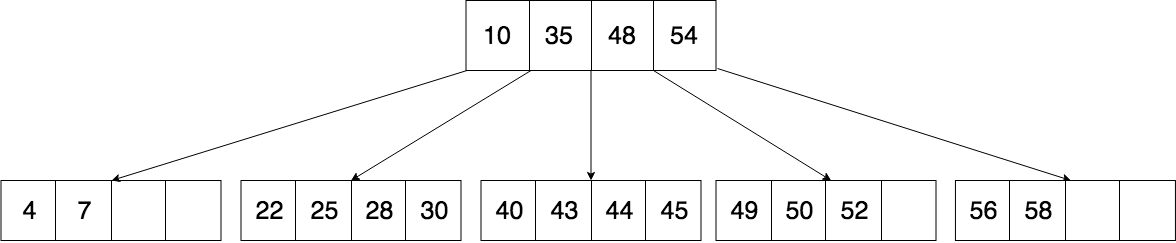
\includegraphics[scale=0.3]{figures/ExampleBTree.png}
    \caption{Example \textbf{B-Tree} with 19 keys. $d = 2$.}
    \label{fig:exB-Tree}
\end{figure}

B+-Trees are a variant of B-Trees: a balanced search tree data structure. B-Trees were first introduced by Bayer and McCreight \cite{bayer1970organization} as a method for indexing records stored in files on secondary storage. Figure \ref{fig:exB-Tree} shows an example B-Tree. Each node in a B-Tree has an order $d$ that determines its capacity, i.e. how many keys it can hold. Each node, except the root, must have between $d$ and $2d$ keys. The root can have between $0$ and $2d$ keys. The pointer between two keys $a$ and $b$ contain keys whose values are greater than $a$ and smaller than $b$.

\begin{figure}[htbp]
    \centering
    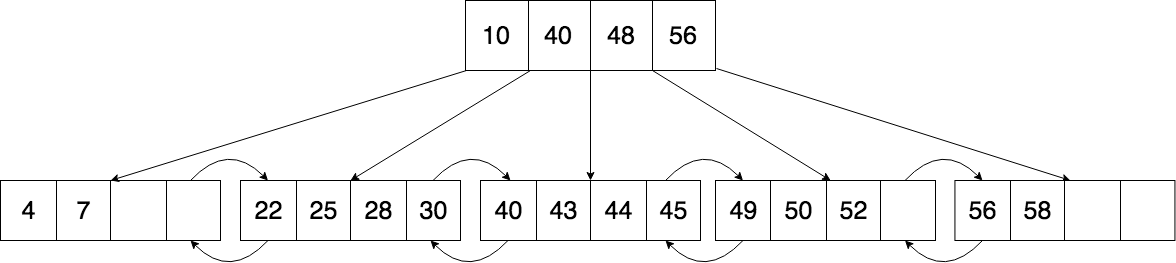
\includegraphics[scale=0.3]{figures/ExampleBplusTree.png}
    \caption{Example \textbf{B+-Tree} with 15 keys. $d = 2$.}
    \label{fig:exB+-Tree}
\end{figure}

B+-Trees vary from their B-Tree counterparts in that their nodes are divided into a \textit{sequence} and \textit{index} set. Figure \ref{fig:exB+-Tree} shows a simple B+-Tree with one internal node (the root) and five leaf nodes holding the keys stored in the tree. The sequence set consists of the leaves of the B-Tree. The index set consists of the internal (non-leaf) nodes. So record keys are found in the leaves, while the internal node contain copies of keys that guide searches to the leaf node containing the desired record. These copies are the result of node splitting. A node split occurs when we try to insert a new key into a full node in order to make room for the new key. After a node split, a copy of the first key in the newly created second node and a pointer to the second node is pushed into the parent node of the first node. This process continues if the parent node is full. Furthermore, traditional B+-Trees have cross-links between leaves. This means the sequence set forms a (doubly) linked list. Restricting keys / records to the leaves leads to simpler deletion and enables fast sequential access of keys. Getting the next key in the sequence of current keys always takes constant time. A survey of B-Trees and their variants, including B+-Trees, was presented by Comer in \cite{comer1979ubiquitous}. 

\subsection{Handling Variable-length Keys} \label{sec:VarLCPKeysMasstree}

\subsubsection{Variable-length Keys and Keys with Long Common Prefixes}

B+-Trees are an excellent data structure for record insertions, updates and retrieval. Any record in a B+-Tree containing a large number of records can be accessed with a few node accesses. Indeed the number of node accesses involved in an operation is a good cost model when analyzing the performance of file-based databases and even main-memory databases. However, it pays to consider the cost of string compares in B+-Trees in the presence of variable length keys that could possibly share long common prefixes. This is because aside from node accesses a fair amount of time is spent looking for the appropriate key in an internal node (to guide search) or in a leaf node (to retrieve the desired record), when searching for a record. The time spent comparing strings is more significant in main-memory databases where the cost of node accesses is relatively low compared to file-based databases.

\begin{figure}[htbp]
    \centering
    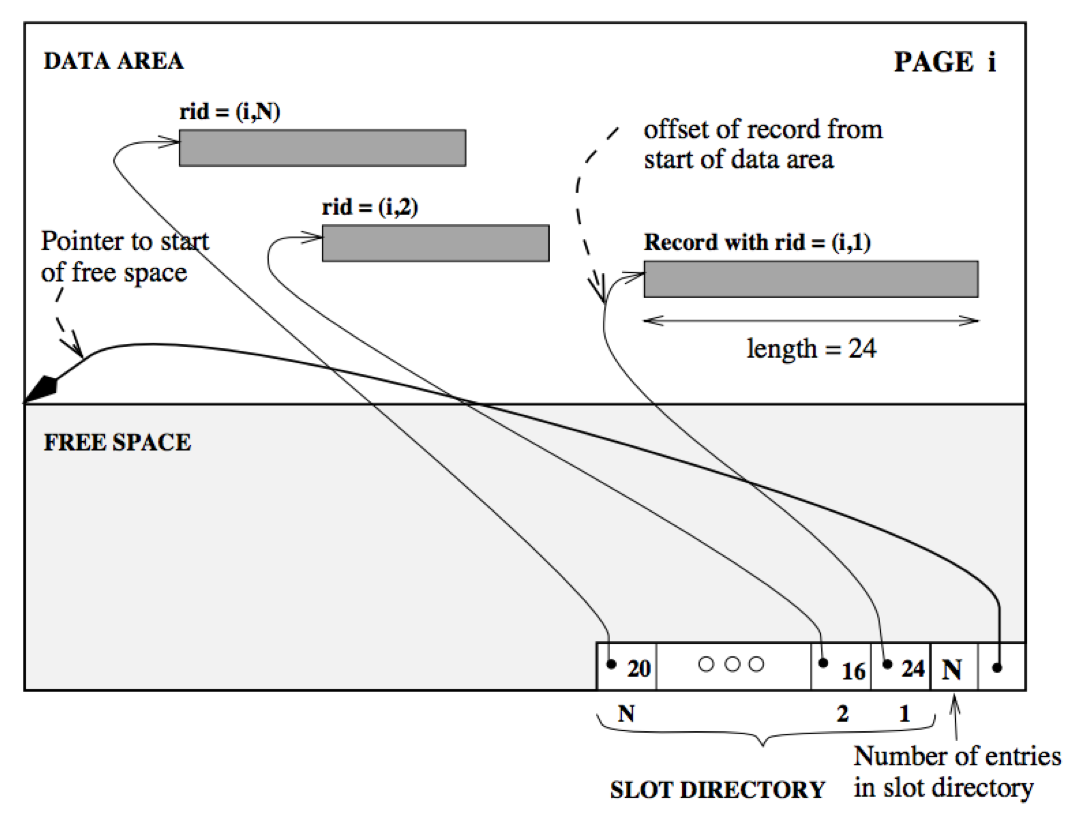
\includegraphics[scale=0.4]{figures/pagevariablelengthkeys.png}
    \caption{Example B+-Tree with $d = 2$.}
    \label{fig:exNodePageB+-Tree}
\end{figure}

Most B+-Tree implementations handle variable-length keys by adding an extra level of indirection. A page/node containing variable length keys in a file-based B+-Tree will look something like Figure \ref{fig:exNodePageB+-Tree} (from page 220 of \cite{ramakrishnan2000database}). VoltDB (a main memory database) also adds a level of indirection when storing long record fields. Figure \ref{fig:voltDBStructure} (from page 48 of \cite{main-mem-dbs}) shows how records are stored in VoltDB's storage layer. Here, record tuples are stored in fixed-sized blocks. If a tuple's field is greater than 8 bytes, it is stored in a variable-size block; the memory address of the item is then stored in the field's location in the tuple instead. In both of the presented cases,  there is a level of indirection involved in finding desired keys within a node. Aside from this being less cache friendly, there is the added complication of maintaining the free area within a node page. Moreover, it is possible that some space could be wasted due to fragmentation within a data page.


\begin{figure}[hbtp]
    \centering
    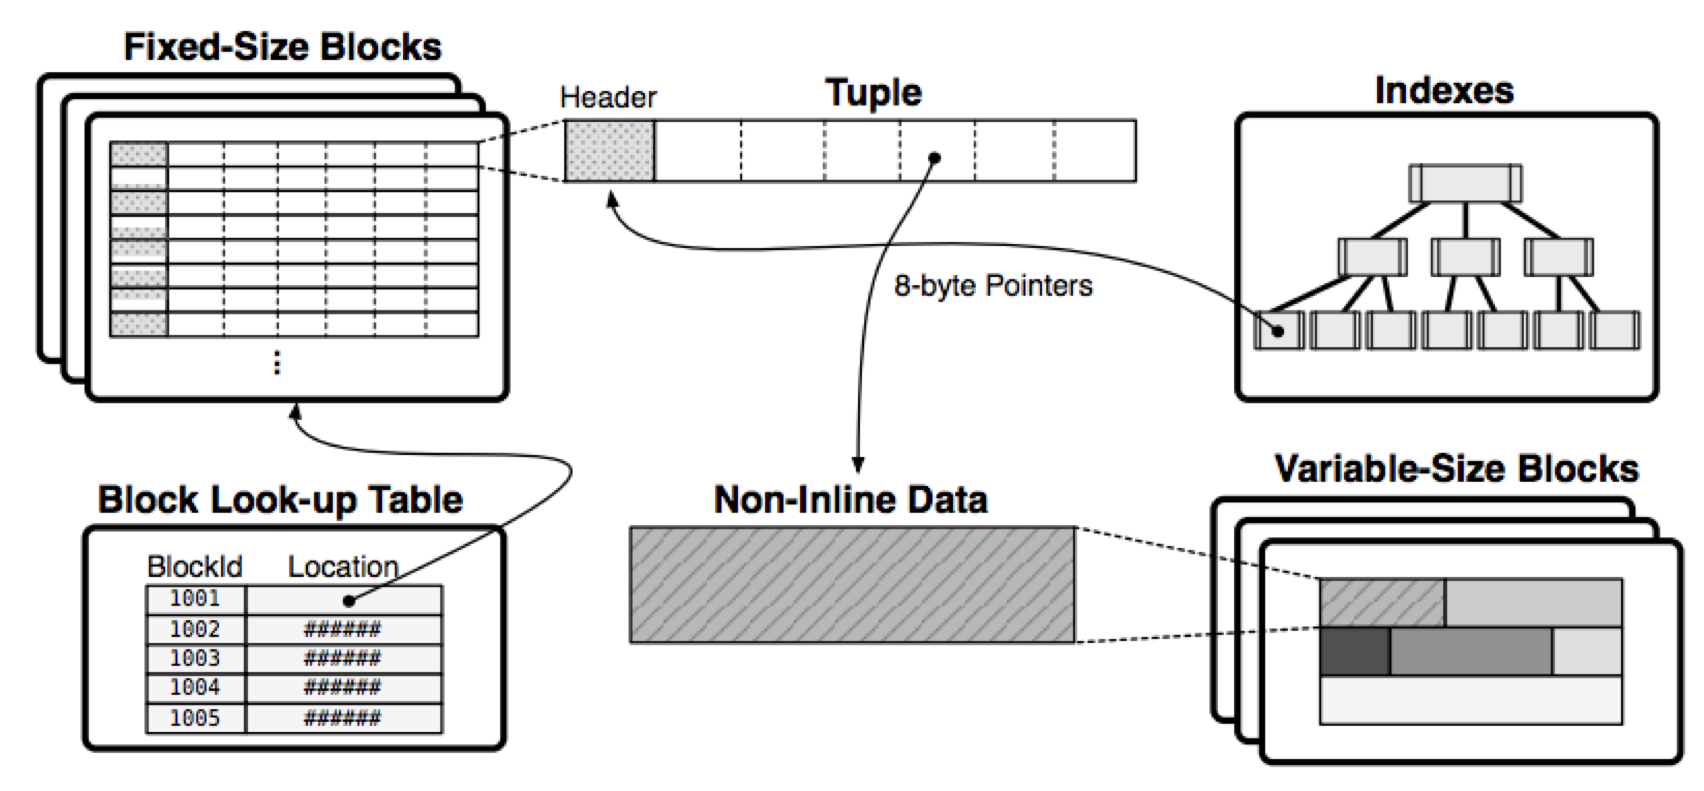
\includegraphics[scale=0.4]{figures/voltdbvariablelengthkey.png}
    \caption{VoltDB storage layout.}
    \label{fig:voltDBStructure}
\end{figure}

\begin{comment}
 VoltDB/H-Store (a main memory database)\cite{main-mem-dbs}, for example, has a fixed-size block pool containing table tuples. If a field is larger than 8-bytes, it is stored in a variable-length block instead. The field in the tuple contains the address of the block instead of the 8-byte data. Traditional file based databases use an "indirection vector"\cite{graefe2011modern} or "directory of slots"\cite{ramakrishnan2000database} with elements of fixed size that point to records in a data area in the page. Each page is a node in the B-Tree. Our implementation follows MassTree's approach instead of the standard approach. An overview of MassTree's datastructure is given below.
\end{comment}
 

\begin{table}[h]
\centering
\label{tab:exampleResourceURLTable}
\begin{tabular}{|l|c|}
\hline
Resource URL                & \multicolumn{1}{l|}{Unique Clients} \\ \hline \hline
/apis/v1/photos/albums      & 753                        \\ \hline
/apis/v1/photos/profile     & 486                        \\ \hline
/apis/v1/info/tutorial      & 1000                       \\ \hline
/apis/v1/info/preferences   & 1000                       \\ \hline
\end{tabular}
\caption{Example of HTTP resource URLs and unique client counts.}
\end{table}

B+-Trees can also run into issues with keys with long prefixes. Consider a web server that periodically processes it server logs and stores in a databases resources requested and the count of how many unique clients requested that resource. An example database table is shown in Table \ref{tab:exampleResourceURLTable}. The corresponding primary B+-Tree index on resource URLs would look like the B+-Tree shown in Figure \ref{fig:urlExampleB+-Tree} (only keys are shown). This simple example is illustrative of how B+-Trees handle long keys that possibly have long common prefixes. Space is wasted saving copies of long keys and performance falls. This is because when searching for any key in the tree, more character comparisons have to be made to determine the lexicographical relationship between two strings that share a long common prefix. 

\begin{figure}[h]
    \centering
    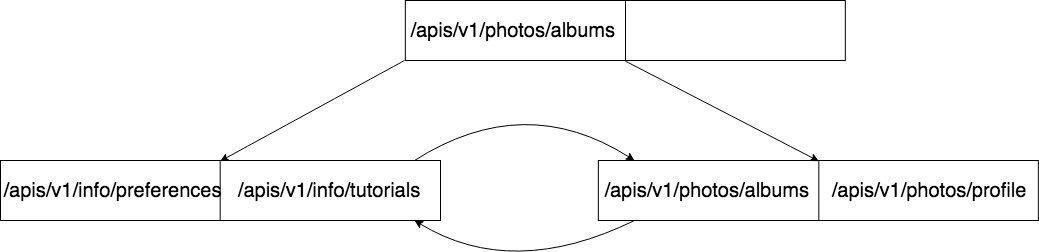
\includegraphics[scale=0.3]{figures/urlexamplebtree.png}
    \caption{B+-Tree index of Table \ref{tab:exampleResourceURLTable} (only keys are shown).}
    \label{fig:urlExampleB+-Tree}
\end{figure}

For the simple example in Table \ref{tab:exampleResourceURLTable}, these issues are not a cause for concern. However, one could imagine a much larger table where there are millions of rows where most keys share long common prefixes. These issues would be intolerable. Even if we take the prefix B+-Tree approach (see \cite{comer1979ubiquitous,ramakrishnan2000database}) - where instead of storing copies of keys in internal nodes, the smallest possible delimiter is used - space could still be wasted if there the common prefixes are long. In Figure \ref{fig:urlExamplePrefixB+-Tree} we see that the root of the prefix B+-Tree index of Table \ref{tab:exampleResourceURLTable} contains the delimiter key \say{/apis/v1/p}. If the largest key to the left of the root and the smallest key to the right of the root shared a longer common prefix, then delimiter key must be longer.


\begin{figure}[h]
    \centering
    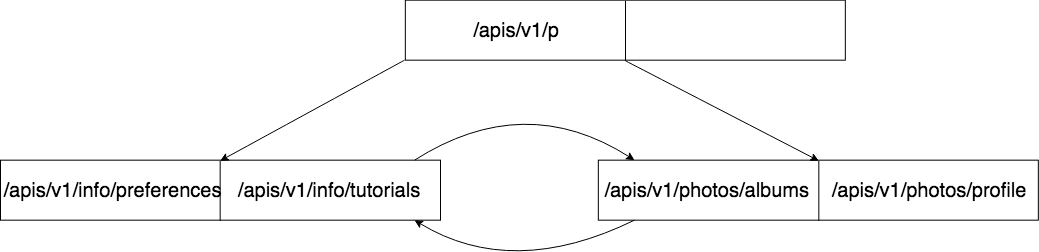
\includegraphics[scale=0.3]{figures/urlexampleprefixbtree.png}
    \caption{Prefix B+-Tree index of Table \ref{tab:exampleResourceURLTable} (only keys are shown).}
    \label{fig:urlExamplePrefixB+-Tree}
\end{figure}


\subsubsection{The solution: Masstree}

Given the aforementioned challenges, our key-value store is based on the Masstree system / data structure. This is to ensure our key-value store can properly handle variable length keys and keys sharing long common prefixes,. 

Masstree \cite{masstree} is an in-memory network key-value storage server that supports range queries. It is also the name of the data structure that the server uses to store key-value pairs. The Masstree data structure is designed to efficiently support arbitrary-length keys, including keys with long common prefixes.  The Masstree system supports \texttt{$get_c(k)$}, \texttt{$put_c(k,v)$}, \texttt{$remove(k)$} and \texttt{$getrange_c(k,n)$} operations. As one might expect, \texttt{get} returns the value associated with a key \texttt{k}. \texttt{put} adds a key-value pair \texttt{(k,v)} into the key-value store or updates the value (\texttt{v}) associated with a key \texttt{k}. \texttt{getrange} returns up to the first \texttt{n} key-value pairs greater than or equal to \texttt{k} in the database. Finally the parameter c is a list of column numbers that allow a client to get or set portions of a key's value. 

The authors of \cite{masstree} describe the Masstree data structure as a \say{trie-like concatenation of B+-Trees}. The structure of a Masstree tree is shown in Figure \ref{fig:MasstreeTreeStructure}. The tree has multiple layers containing one or more B+-Tree. The root layer contains at most one B+-Tree, the second layer contains at most $2^{64}$ trees - one for every possible key the first layer can have - and so on. Each B+-Tree and layer is responsible for some 8-byte slice of a key. Masstree's B+-Trees consist of interior nodes and border nodes(see Figure \ref{fig:MasstreenodeDS}). 

\begin{figure}[htbp]
    \centering
    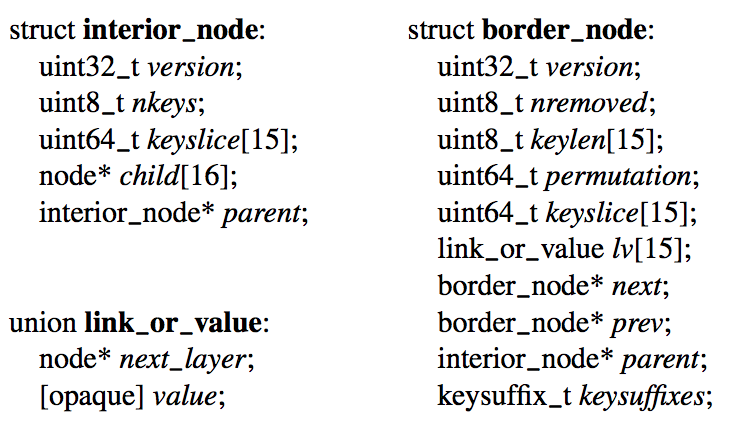
\includegraphics[scale=0.50]{figures/masstreenodestructures.png}
    \caption{Masstree Node Data Structures \cite{masstree}}
    \label{fig:MasstreenodeDS}
\end{figure}

Border nodes are similar to traditional B+-Tree leaf nodes. They have cross-links (to aid the \texttt{getrange} operation), keys and key values. However, Masstree's border nodes are unique in that their keys are identified by an 8-byte key slice and a key length. This means that a single Masstree B+-Tree can represent multiple (at most 10) keys with each key slice. At most 9 different keys for every possible prefix of the keyslice (keys with length 0 to length 8) and a 10th key in the event that there is a key suffix or a link to the next layer. Not all key slices can have 10 different keys. A key slice with no null bytes can have only two different keys. A key with a null byte at the end can have three different keys. Moreover, for each key in a border node, there is a value or a link to a B+-Tree in the next layer. Whether a key points to a value or another B+-Tree depends on the value of its key length field. If a key's key length is greater than 8, then the key has a suffix and a value or has a link to another layer instead of a value. 

\begin{figure}[hbtp]
    \centering
    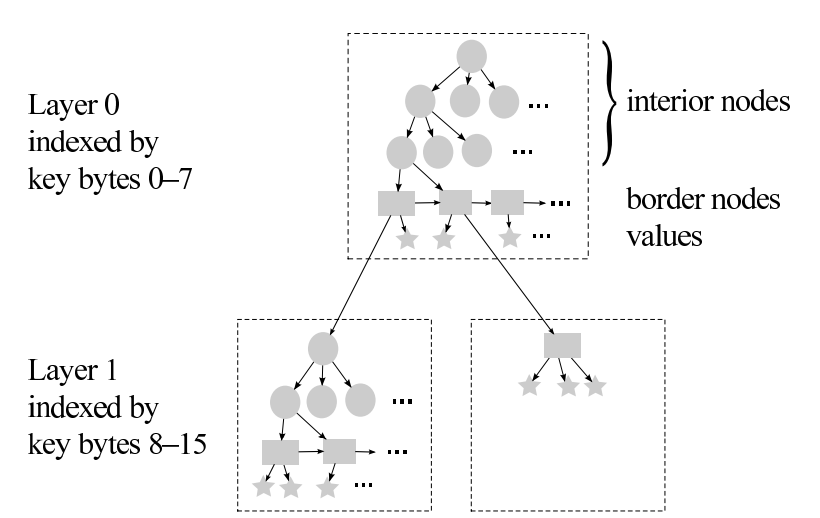
\includegraphics[scale=0.50]{figures/masstreedatastructure.png}
    \caption{Masstree Tree Structure \cite{masstree}}
    \label{fig:MasstreeTreeStructure}
\end{figure}

MassTree border nodes also contain keysuffix data structures in the event that a key's suffixes aren't shared by any other keys with the same prefix. That is, if we have the keys \texttt{"AB"} and \texttt{"ABCDEFGH!"} in our key-value store, there is no need to create a second layer to index the last byte of the second key. On the contrary, we store \texttt{"AB"} (2 bytes) and \texttt{"ABCDEFGH!"} (9 bytes) with their appropriate key slices and key lengths in a B+-Tree with a single node (layer 0). Then we set the keysuffix for the latter of the key slices to be \texttt{"!"}. However, if we have another key \texttt{"ABCDEFGH*"}, key slice \texttt{"ABCDEFGH"} must now point to a new layer. In addition, the string whose suffix is $"!"$ is inserted in the new layer with its original value and the new string whose suffix is \texttt{"*"} is inserted in the new layer with its value. Generally, if a key is $8h$ bytes long, its value will be stored at layer $x$ where $x < h$. So, if a key is 8 bytes or less, its value will be referenced by a keyslice in the root layer's B+-Tree. If a key is 40 bytes long, its value will be stored in one of layers 0 to 4. This is because key suffixes can be stored in a bordernode, if no other prefixes of the full key share in the keyslices up to a layer and part of the suffix. The keysuffix data structure means that unnecessary layers are not created when there are many relatively long keys that do not share common prefixes. On the other hand, if there are long keys that share common prefixes, then multiple layers (relatively small layers) would be responsible for a portion of the common prefix. Which keeps retrievals fast as shown in the Evaluation Section \ref{sec:Evaluation}.

\begin{comment}
Operations in MassTree can benefit from cache-locality compared to typical B+-Tree schemes where variable length keys are handled by an extra level of indirection (areas outside the tree to store long keys) (reference???). Operations also benefit by reducing space costs associated with storing multiple keys with common prefixes separately.
\end{comment}

\section{System} \label{sec:Our System}

\subsection{Operations} \label{sec:kvstore operations}
Our overall system is implemented as a C programming language library and currently exposes the following operations:
    
    \begin{itemize}
        \item \texttt{KVStore\_T KV\_NewKVStore(void);}
        \item \texttt{Bool KV\_Put(KVStore\_T kvStore, KVKey\_T key, const void* value);} %%% update to void in code.
        \item \texttt{const void* KV\_Get(KVStore\_T kvStore, KVKey\_T key);}
    \end{itemize}

\texttt{KV\_NewKVStore} returns a newly created key-value store instance. \texttt{get} retrieves the value associated with the given key in the store. \texttt{put} adds a key-value pair to the key-value store or updates the value associated with an existing key. Our key type \texttt{KVKey\_T} is created from an array of chars with its specified length. The return type of put will be updated to void because put should always succeed, unless perhaps memory allocation fails (which is extremely unlikely).

\subsection{Architecture Overview}

Our system is a client of two internal libraries: a \texttt{B+-tree library} and a \texttt{Bordernode library}. The B+-Tree library enables the creation of B+-Trees and operations on those B+-Trees. The Bordernode library implements a variant of Masstree's \cite{masstree} bordernodes (nodes at the border of two btree layers). See section \ref{sec:B+-tree implementation} for more details. We also implement a \texttt{utility library} for some common definitions and operations used across the different libraries. 

\begin{comment}
    how much detail to go here? 
    
    architecture diagram?
\end{comment}

\subsection{B+-Tree Implementation} \label{sec:B+-tree implementation}


Our system's B+-Tree data structure is similar to the traditional B+-Tree. However, we do not use cross links between leaf nodes in our implementation, but rather add a new independent auxiliary data structure called a B+-Tree cursor. The B+-Tree cursor can be thought of as an array of node pointers and corresponding pointers to entries within each node (Figure \ref{fig:exB+-Tree}). Each entry in an internal node consists of a key and the pointer to its right. The first entry has no key associated with it. It is simply a pointer. In leaf nodes entries consist of keys and pointers to the record/value they are associated with. The first element of the cursor points to an entry in the root node. The second element in the cursor points to an entry in the child of the entry pointed to in the root, and so on until an element of the cursor points to an entry in a leaf node. The cursor therefore points to all the entries (and nodes) in the unique path from an entry in the root to an entry in a leaf node. 

\begin{figure}[h]
    \centering
    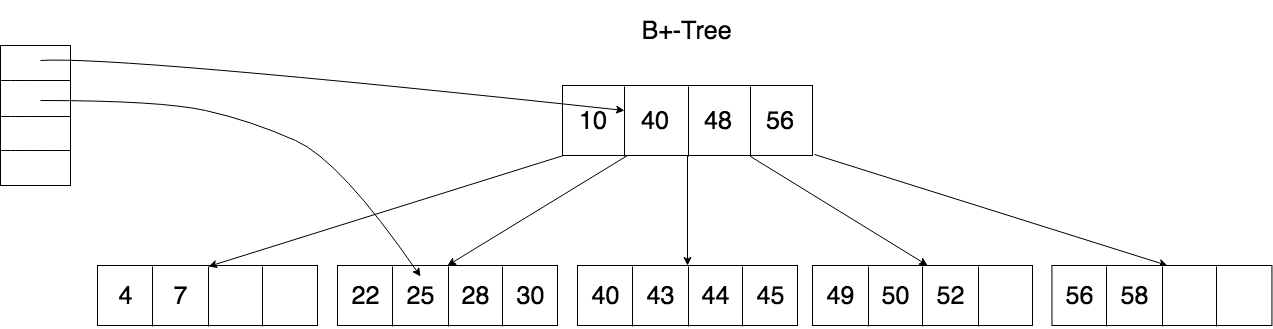
\includegraphics[scale=0.30]{figures/BtreeCursor.png}
    \caption{B+-Tree Cursor Pointing at Key 25.}
    \label{fig:exB+Cursor}
\end{figure}

It is important to know that we were inspired to use this B+Tree with cursor concept from SQLite \cite{SQLite}. SQLite's B-Tree implementation supports both B+-Trees (called B*-Trees in their documentation) and B-Trees. B+-Trees are used as what SQLite calls "Table B-Trees", while B-Trees are used as "Index B-Trees". See \cite{SQLiteFileFormat} for SQLite's database file format documentation. The beauty of this data structure is that it enables \textbf{both} fast sequential gets and puts. More specifically, a sequential get or put operation takes amortized constant time. If these assertions are true, insertion of a set of sorted key-value pairs takes linear time and partially sorting a set of keys involved in a series of get and/or put operations can lead to large performance gains. It would also mean that databases using this B+-Tree scheme can reduce the time it takes for operations that build trees / tables from sorted data e.g. failure recovery, data replication. Moreover, if queries come in batches, they can be partially sorted to reduce processing time. 


\begin{comment}
internal nodes lead search can have high fanout and take relatively less space. makes deletion easier.
cross links guarantee constant time. 

With very large d, All this means we fetch few files when searching for a key or when 

ADD figure of B+-Tree and B-trees and reference it.

Reference insertion and deletion algorithms.

THANK AURELE FOR WORK on this implementation

Draw picture of array and trees.
draw graph of cursor.
Proof of amortized constant time.
refer to both.

2 log n worst case time is what happens in a recursive implementation

examples of building b-tree from sorted or partially-sorted data.

algo for B+-Tree cursor insert.

ubiquitous b-tree - general info about b-trees and variant
modern b-tree techniques = more detailed exploration of b+-trees for database exploration
dbms book - algo for trad b+-trees

figures don't show all details, like other information in nodes / cursor
\end{comment}


\subsubsection {B+-Tree Cursor and Operations}

The B+-Tree Module interface has various methods for operating on B+-Trees, including: \texttt{MoveToFirst}, \texttt{MoveToNext} and \texttt{MoveToPrevious}, However, in this section we will focus on the \texttt{MoveToKey}, \texttt{MoveToNext} and \texttt{PutRecord} operations on B+-Trees with a FANOUT (maximum number of keys per node) of two. The FANOUT can be varied and in our implementation it is set to a default value of 15, similar to the node FANOUT of Masstree \cite{masstree}. 

\begin{figure}[h]
    \centering
    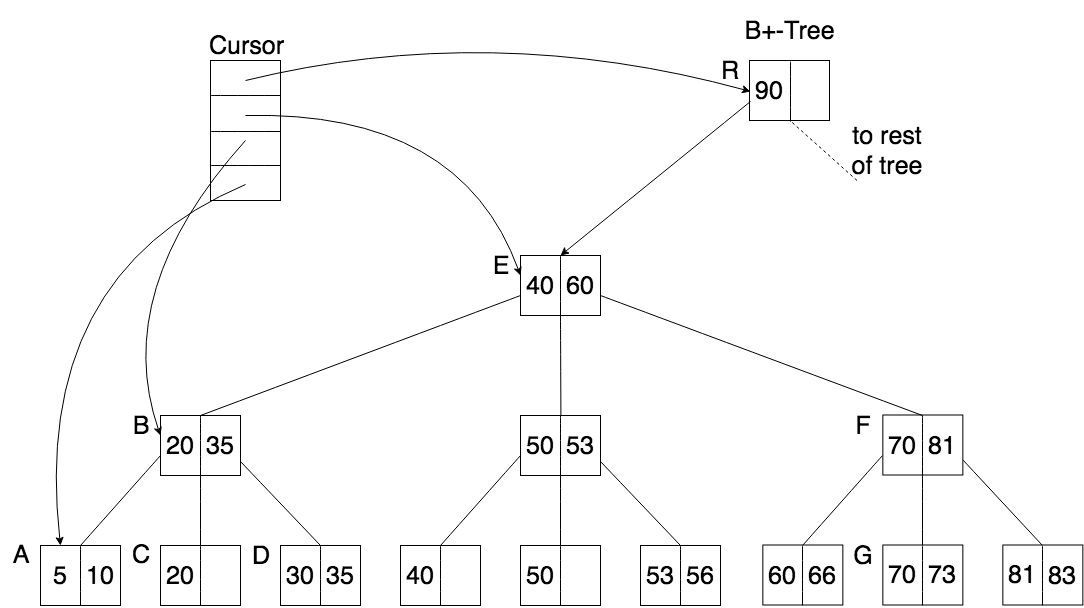
\includegraphics[scale=0.30]{figures/CursorAt5.png}
    \caption{B+-Tree Cursor Pointing at Key 5.}
    \label{fig:exB+Cursor5}
\end{figure}

\texttt{MoveToKey} and \texttt{MoveToKey} operations are simple if the desired key is in the same node. We just search for the correct key within the current node. For example, if the cursor is at key 5 in Figure \ref{fig:exB+Cursor5}, a \texttt{MoveToNext} or \texttt{MoveToKey(10)} operation should simply move the cursor to the next entry in the node, entry 10. However, if the desired key resides in a leaf node one or more nodes away from the current leaf node, there is more work involved. In the traditional implementation of B+-Trees, a move-to-next operation simply uses the cross-links between leaf nodes to get to the next node, and consequently the next key. Nevertheless, a random search always starts from the root. In our B+-Tree implementation a random search (or next operation to an entry in a sibling node) starts from the current leaf node and ascends and descends through the tree \textbf{as needed} to get to the desired key. 

\begin{figure}[h]
    \centering
    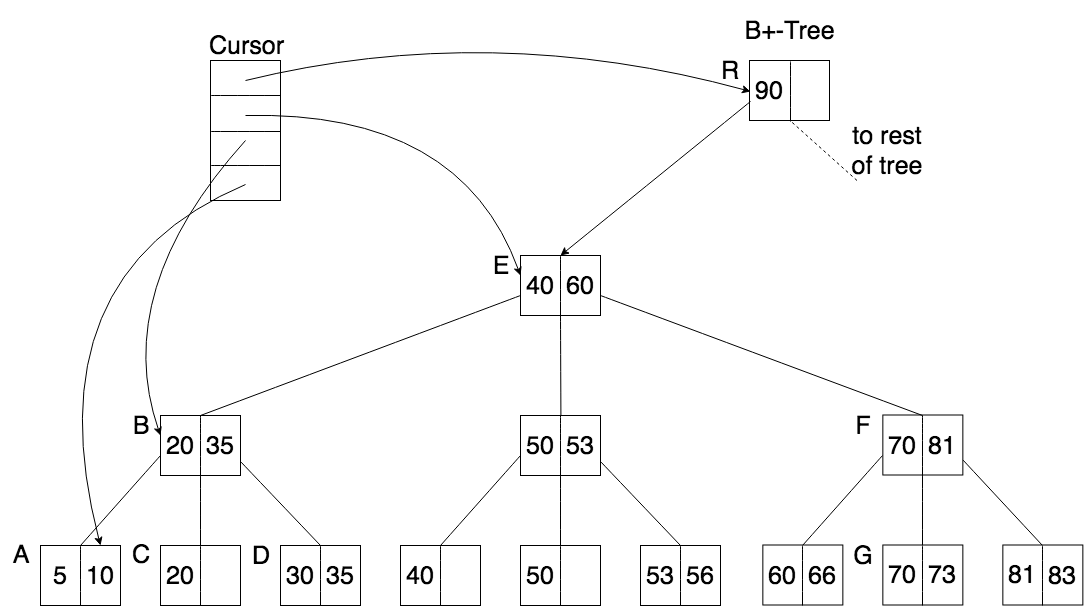
\includegraphics[scale=0.30]{figures/CursorAt10.png}
    \caption{B+-Tree Cursor Pointing at Key 10.}
    \label{fig:exB+Cursor10}
\end{figure}

\begin{figure}[h]
    \centering
    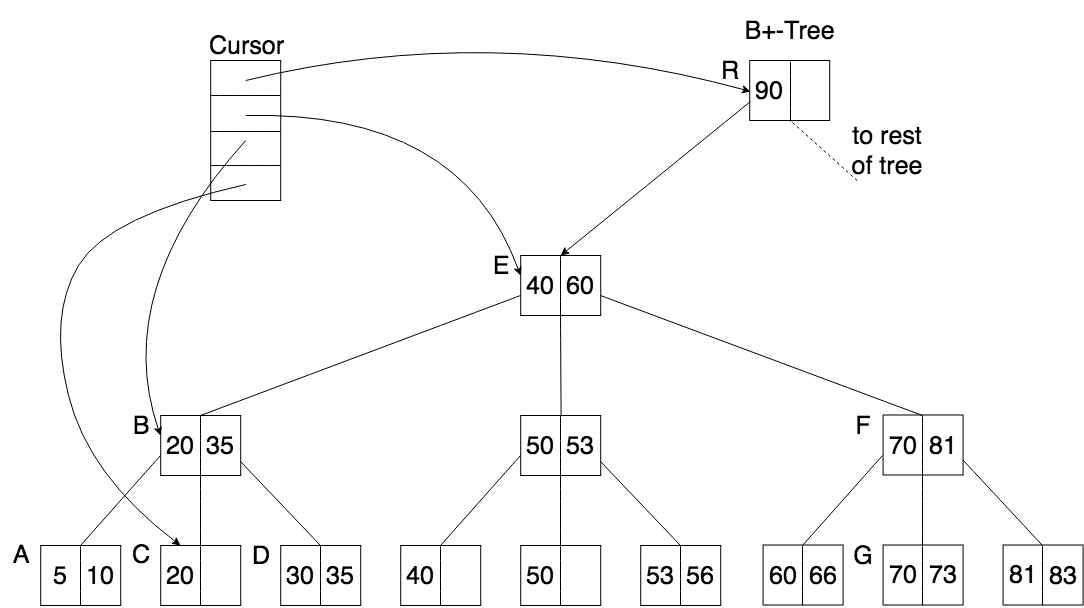
\includegraphics[scale=0.30]{figures/CursorAt20.png}
    \caption{B+-Tree Cursor Pointing at Key 20.}
    \label{fig:exB+Cursor20}
\end{figure}


More specifically, in the case of a \texttt{MoveToNext} operation, the cursor first moves up to the closest ancestor node that it is not pointing to the last entry within. i.e. an ancestor node for which the cursor can move to the next entry within. Afterwards, the cursor then sets the pointer at that level to the next entry in the node and then descends to the entry's smallest leaf child. For example, consider a \texttt{MoveToNext} operation from key 10 (Figure \ref{fig:exB+Cursor10}), this moving the cursor's last pointer from entry 10 on node A to entry 20 on node C (Figure \ref{fig:exB+Cursor20}). To do this, the cursor first ascends to node B. Then it moves its entry pointer for that level to the next entry in node B. Finally it descends to the current entry in node B's smallest leaf child. If the cursor was originally at the last entry in node B, it would have to keep ascending till it either reaches the root or a node where its pointer for that node/level was not previously pointing to the last entry in the node. For example, if the cursor was at key 35 (node D), a move to the next entry (key 40) entails moving up to node E, moving the entry pointer in that node to the next entry and then descending to the left most leaf child.

For a random search, the cursor has to move up to the closest node that is definitely an ancestor of the desired search key. This is a node where the search key is greater than or equal to its first entry and strictly smaller than its last entry. The only exception to this rule is the root. The root is an ancestor of every node in the tree. After a definite ancestor of a key has been found the cursor can then descend down the tree from this node to the desired leaf entry. For example, let the cursor be at key 20 (Figure \ref{fig:exB+Cursor20}). What happens when \texttt{MoveToKey(50)} is called? To move to key 50, the cursor first ascends to node E. It does not go beyond node E as 50 is in between node E's smallest and greatest key. We then descend to node H then node I which contains key 50 (Figure \ref{fig:exB+Cursor20}). What if a call is then made to \texttt{MoveToKey(73)}? In this scenario, the cursor ascends all the way to the root R, and then descends to node E then node F and then node G. The cursor then points at key 73 (Figure \ref{fig:exB+Cursor73}). The cursor has to ascend all the way to node R (the root) because it is impossible from simply looking at node E's entries to know for sure that node E is definitely an ancestor of key 73. All node E's entries can inform us is that children of its greatest entry are greater than or equal to 60. It is possible that another child of E's parent could be the ancestor of key 73. This would be the case if the first key in node R is less than 73. This is an example of the worst case of random search with the B+-Tree scheme. In the worst case, a \texttt{MoveToKey} call takes time proportional to $2 log N$. $log N$ time to ascend to the root and $log N$ time to descend from the root to the apropriate leaf node. This is in contrast to random search in the traditional B+-Tree scheme which always takes time proportional to $log N$. However it is important to note that the cost to ascend will not be significant as most (if not all) of the nodes in the ascend path are likely to be in cache (more specifically higher levels of cache memory) because they have been recently visited. On the other hand, whenever we carry out a random search for a nearby node, we benefit from not needing to ascend to the root and from most of the nodes we visit being in higher levels of cache memory. 

\begin{figure}[h]
    \centering
    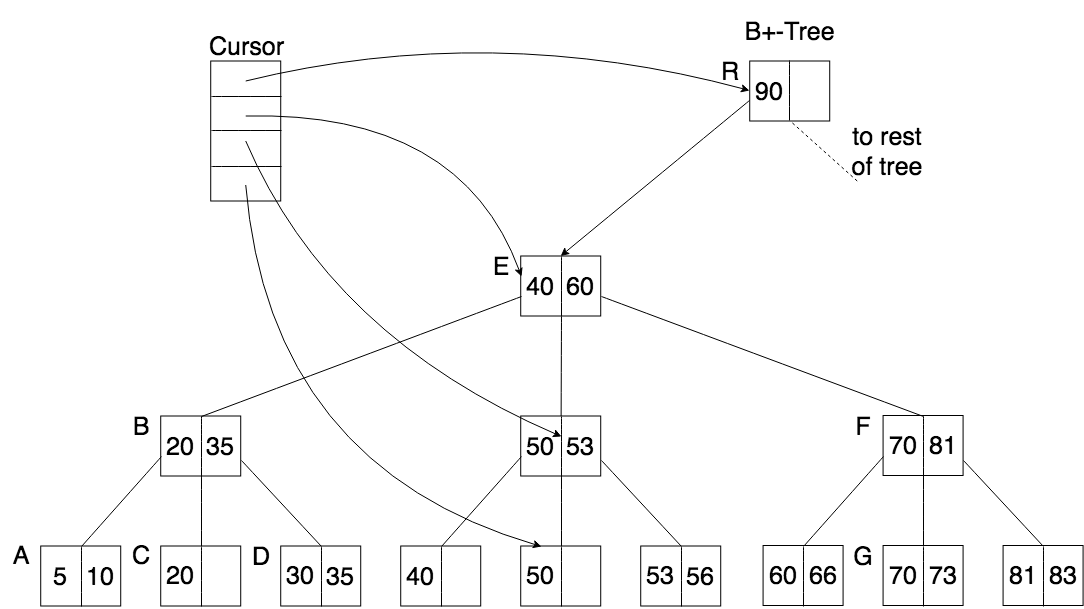
\includegraphics[scale=0.30]{figures/CursorAt50.png}
    \caption{B+-Tree Cursor Pointing at Key 50.}
    \label{fig:exB+Cursor50}
\end{figure}


\begin{figure}[h]
    \centering
    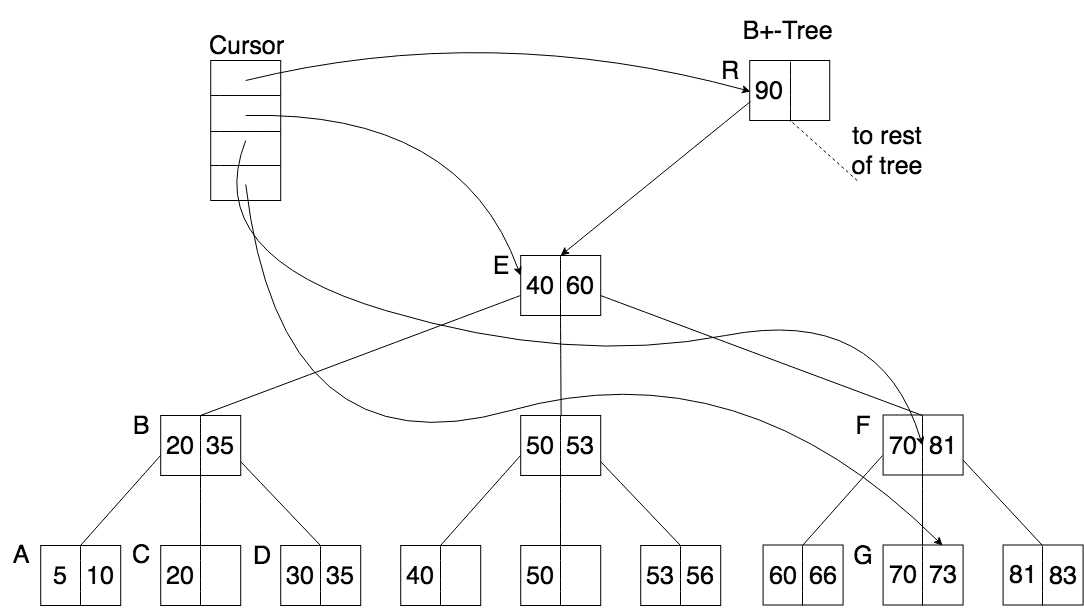
\includegraphics[scale=0.30]{figures/CursorAt73.png}
    \caption{B+-Tree Cursor Pointing at Key 73.}
    \label{fig:exB+Cursor73}
\end{figure}


Sequential (next) operations are fast as well. Most of the time they entail simply moving to the next element in a node, a few times they entail a jump from a node to its right sibling node which often involves fewer node accesses and occasionally, in the worst case, involves $2h$ node accesses, where $h$ is the height of the tree. Inserts can benefit from using this scheme (i.e using a cursor that remembers its current location and the path to it). With sequential inserts, most of the time, the current node has enough space for the next key. Sometimes, we need to split the node (node splits are described briefly in \ref{sec:indexB+-trees}). Most of the time, a single split is enough. Sometimes the split propagates upward to one or more nodes. Occasionally, a node split propagates up multiple levels. As a result, we expect that a sequential put or random put \textbf{near} the cursor's current location will be quick and simply involves the cost of moving to a nearby location and inserting a key; both of these steps (move and put) are often fast if the key to be put into the tree is near the key the cursor is pointing to.

\begin{comment}
   Nevertheless, it is unlikely that, in a series of random searches / move-to-key calls, the desired key is always very far from the cursor's current position. Sure, except due to caching doing this constantly is very fast.
\end{comment}
 
 

In conclusion, aside from reducing the number of node accesses needed in move and put operations, the B+-Tree with cursor scheme benefits highly from cache-locality when the cursor does not move too far. It is less likely to access unnecessary nodes in the path from parent to the desired key, rather it is more likely to revisit previously visited nodes. For example, when traversing the tree from keys 5 to 35 (imagine a range query or sequential updates), our B+-Tree with cursor scheme visits only nodes A, B, C and D. Note we visit node B FANOUT (two) times. This implies that if a sequence of operations is partially sorted by key we can experience massive performance gains, subject to how much we sort the sequence of operations. It is important to note that SQLite \cite{SQLite} (which uses this B+-Tree with cursor scheme) does not always benefit if the cursor is at a key close to a search key. Indeed, SQLite's \texttt{sqlite3BtreeNext} function behaves similarly to our \texttt{MoveToNext} function: most of the time the next key would be in the current node and SQLite's cursors only ascends the tree as needed. Nevertheless, SQLite's \texttt{MoveTo} function always starts searching for the desired key from the root, unless the cursor is already at the correct position. This is in contrast to our implementation of \texttt{MoveToKey} which never begins search from the root. Therefore, a partially random sequence of operations would be expected to execute as quickly as a random sequence of operations and experience no performance gains in SQLite. 

\subsubsection {Why Sequential Operations are Amortized Constant Time}

\begin{figure}[h]
    \centering
    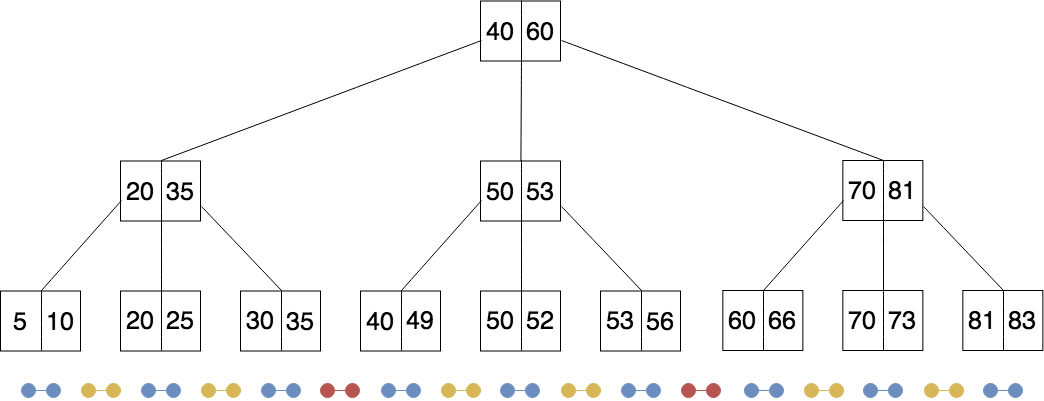
\includegraphics[scale=0.30]{figures/amortizedtimenextexample.png}
    \caption{Example B+-Tree with 18 keys and height 3 (cursor not shown). When sequentially visiting all keys in the B+-Tree, there are 17 total next operations: 9 blue next operations, 6 yellow next operations and 2 red next operations.}
    \label{fig:amortizedanalysisheight3}
\end{figure}


In this section, we will investigate the claim made in \ref{sec:indexB+-trees} that a sequential get or put operation takes amortized constant time. Figure \ref{fig:amortizedanalysisheight3} gives an intuition for why this might be the case. Traversing through the tree in Figure \ref{fig:amortizedanalysisheight3} from key 5 to key 83 takes 17 next operations. Most (about half) of these  operations are the low cost blue next operations.These blue next operations cost little as they simply involve moving the cursor to the next element in the node and involve zero extra node accesses. The other (roughly) half of next operations require a jump from one node to another. Most of these next operations require the cursor moving up only one level and then down to reach the sibling node containing the next entry. These are the yellow operations which require only two node accesses. Few of these next operations require the cursor moving up to the root and then down to the next entry in the sibling node. These are the red next operations, the most costly next operations.



\begin{figure}[p]
    \centering
    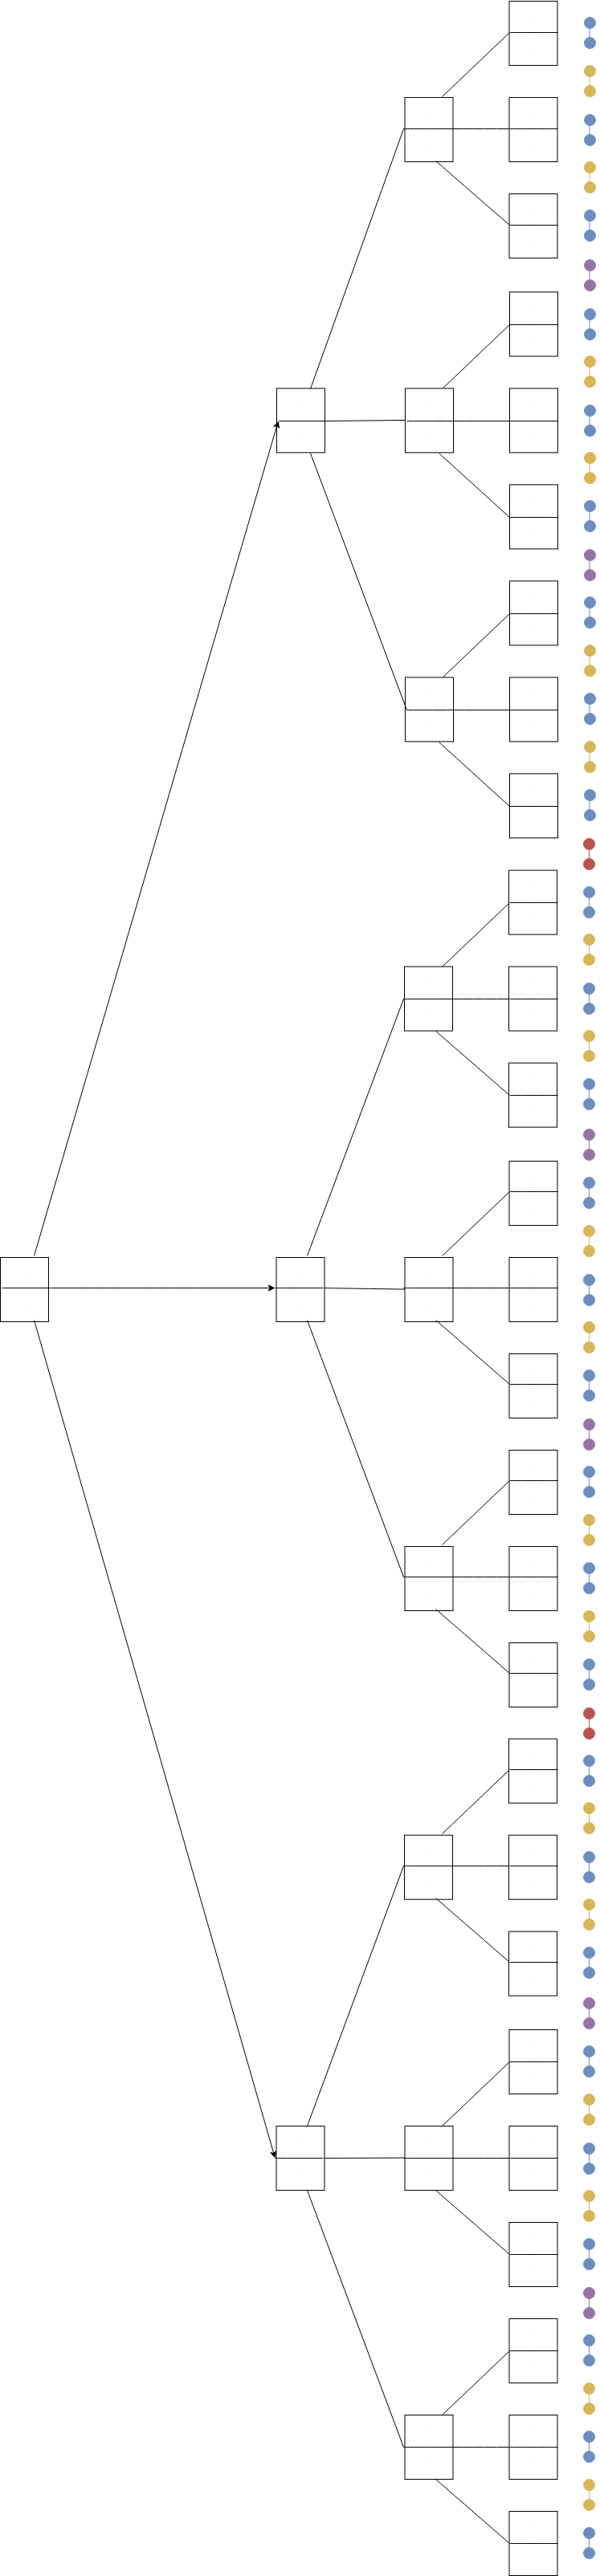
\includegraphics[scale=0.18]{figures/amortizedtimenextexamplehugerotated.png}
    \caption{Example B+-Tree with 54 keys and height 4 (cursor not shown). When sequentially visiting all keys in the B+-Tree, there are 53 total next operations: 27 blue next operations, 18 yellow next operations, 6 purple operations and 2 red next operations.}
    \label{fig:amortizedanalysisheight4}
\end{figure}

For our tree with 18 keys, in order of costliness there are:

    \begin{itemize}
        \item 2 red operations
        \item 6 yellow operations
        \item 9 blue operations
    \end{itemize}

If our tree was a level deeper, as in Figure \ref{fig:amortizedanalysisheight4}, in order of costliness there are:

    \begin{itemize}
        \item 2 red operations
        \item 6 purple operations
        \item 18 yellow operations
        \item 27 blue operations
    \end{itemize}
    
We see that the most costly jumps occur $2 * 3^0$ times, the next most costly operations occur $2 * 3^1$, the next most costly operations occur $2 * 3^2$ times and so on. The least costly operations, however, occur $3^h$ times where $h$ = the height (number of levels) of the tree. This implies that the most costly operations which are proportional to $log N$ where $N$ is the number of entries in the tree occur very infrequently. If each next operation was logarithmic on average, we will expect that most of the next operations are proportional to $log N$. Not only is this not the case, but we see that the more costly an operation, the (exponentially) less likely it is to occur. Put another way, a fraction of the time a next operation requires that we jump to the next node.  When jumping from a node to the next, a majority of the time moving up one level and then back down is sufficient. A fraction of the time when we jump between two nodes, we need to move up two levels and then back down. An even smaller fraction of the time we need to move up three levels and then back down, and so on and so forth.  

With this intuition we can find an upper bound of the average cost of a next operation for a tree of any height:

\begin{equation} \label{eq:TnextaveExp1}
    T_{ave} < c + \frac{2}{F} + \frac{4}{F^2} + \frac{6}{F^3} + ... = c + \frac{2 \times 1}{F} + \frac{4 \times 2}{F^2} + \frac{6 \times 3}{F^3} + ...
\end{equation}

\begin{equation} \label{eq:TnextaveSeries}
    T_{ave} < c + \sum_{i=0}^{\infty} \frac{2i}{F^i} 
\end{equation}

where $F$ is the FANOUT - maximum number of keys - in each node in the B+-Tree.


In Equation \ref{eq:TnextaveExp1}, we see that a next operation always takes some constant plus 2 node accesses $\frac{1}{F}$ of the time, plus 4 node accesses $\frac{1}{F^2}$ of the time and so on. The frequency of costly operations decreases exponentially. This is an upper bound because in reality the probability of any jump is $\frac{1}{F}$, low cost and high cost jumps included. So this means that in reality, the most frequent lowest cost jumps occur less than $\frac{1}{F}$ of the time, the next lowest cost jumps occur less than $\frac{1}{F^2}$ of the time and so on. 

The series in equation \ref{eq:TnextaveSeries} is the product of an \textbf{arithmetic} and a \textbf{geometric} series. It is an \textbf{arithmetico-geometric} series. We know that the sum from an arithmetico-geometric series is given by \cite{riley2011foundationmaths}:

\begin{equation} \label{eq:arith-geometricSeries}
    S = \sum_{n=0}^{\infty} (a + n d)r^n = \frac{a}{1-r} + \frac{rd}{(1-r)^2} 
\end{equation}


where $r < 1$.

Equation \ref{eq:TnextaveSeries} can be simplified with \ref{eq:arith-geometricSeries} to yield:

\begin{equation} \label{eq:TnextaveResult}
    T_{ave} < c + \frac{2F}{(F-1)^2} 
\end{equation}


From Equation \ref{eq:TnextaveResult}, we see that the average cost of a next operation for a tree of any height with fanout F is upper-bounded by some small cost plus $\frac{2F}{(F-1)^2}$ node accesses. This shows two things. Firstly, a next operation does not take logarithmic time (is not proportional to the height of the tree), but rather takes amortized constant time. Secondly, the cost of a next operation is inversely proportional to the FANOUT $F$ of the nodes in the tree.

Given the previous analysis, we can also find an upper bound for the cost of a sequential put operation. i.e. a put operation where the key=value pair to be updated or inserted is to be placed beside the current key. We know that the cost of a sequential put operation is the cost to move to the appropriate node (same node or sibling node) plus the cost of inserting the entry. We already know that the cost to move to the next key (next appropriate node) is less than the upper bound in Equation \ref{eq:TnextaveResult}. We know that inserting a key-value pair in a node takes some constant and might involve node splits. How often are node splits? Imagine a sequence of sequential inserts, where each key is not present in the tree. Most of the time a node will have space for an insert and not require any node splits (see \ref{sec:indexB+-trees}). A fraction of the time (proportional to $\frac{1}{F}$) there is a node split. A fraction of the time when there is a node split it propagates up to the next level, a fraction of the time when a split propagates by one extra level it propagates another level, and so on.  

We can find the average cost to insert a new key into a node by simplifying the following inequality:

\begin{equation} \label{eq:TinsertAtLocation}
    T_{ins} < c + c_{split}(\frac{1}{F} + \frac{2}{F^2} + \frac{3}{F^3} + ...)
\end{equation}

That is the cost of inserting a new key-value pair is less than some constant plus the cost of a split that occurs at most some time proportional to $\frac{1}{F}$ plus the cost of two splits that occurs at most some time proportional to $\frac{1}{F^2}$ and so on. The constant$c_{split}$ is to account for the fact that splits occur in proportion to the fractions involved in the geometric series.

\begin{equation} \label{eq:TinsertAtLocationResult}
    T_{ins} < c + c_{split}\sum_{i=0}^{\infty} \frac{i}{F^i} = c + \frac{c_{split}F}{(F-1)^2} 
\end{equation}

Using Equation \ref{eq:arith-geometricSeries} we solve the arithmetico-geometric series in Equation \ref{eq:TinsertAtLocation} to find an upper bound on the cost of insertions.

Putting equation \ref{eq:TnextaveResult} and equation \ref{eq:TinsertAtLocationResult} together an upper bound on the cost of a sequential insert and, consequently, a sequential put is:

\begin{equation} \label{eq:Tseqput}
    T_{seqput} < T_{ins} + T_{ave} = c_1 + \frac{2F}{(F-1)^2} + c_2 + \frac{c_{split}F}{(F-1)^2} 
\end{equation}


As we can see from equation \ref{eq:Tseqput}, the time it takes for a sequential put is lest than some constant inversely proportional to the fanout $F$. Therefore sequential puts also take amortized constant time. 

\begin{comment}
If we have d to the (h) keys, in the best case next takes constant time, in the worst case it take time proportional to h, as we have to go to the root and back down. however, if we have n random gets or get next operations this happens once every n times.
\end{comment}

\subsection{Key-value Store Implementation} \label{kvstore implementation}

In this section we discuss our key-value store implementation. Our key-value store is implemented in the C programming language as a library (called KVStore). It currently supports the operations outlined in section \ref{sec:kvstore operations}. It is a client of the B+-Tree module \ref{sec:B+-tree implementation} and the BorderNode module. Our B+-Tree module as is can only handle fixed length 8 byte keys. Therefore it must be extended to handle variable length keys. As mentioned in section \ref{sec:VarLCPKeysMasstree}, databases and storage systems that use B+-Trees tend to handle variable length keys by adding a level of indirection between a node's slot array and the record / record key in the node's data area; we also saw how B+-Trees are not optimized for handling keys with long common prefixes. We discussed how Masstree effectively handles variable-length keys and keys with long common prefixes. As a result, our KVStore Module is based on Masstree. It is also a trie-like concatenation of B+-Trees.

\begin{comment}
    For example, in SQLite (where records are stored in files by default), B+-Trees are used as a Table index, while ... index, and each node is a page on disk, variable length keys are .... Other external storage based databases use a similar / different approach (check databasemanagement book and other modern b-tree techniques). With main memory databases there is more flexibility to try different approaches. For example, this system handles variable length keys by this. That system handles variable length keys by that.
    
    Mainmemdbs page 49/52 h-store uses variable sized blocks. modern b-tree techniques indirection vector page 236. 220 database management textbook 220
\end{comment}

\subsubsection{Key-value Store Module and BorderNode Module}

Our key-value store module is based on Masstree. It can be viewed as a serial re-implementation of Masstree. However, there are a few differences. As mentioned previously, it is a client of the B+-Tree module \ref{sec:B+-tree implementation}. We also made the decision to implement border nodes separately from the B+-Tree; our B+-Tree's leaf nodes are not border nodes. Our B+-Tree module's leaf nodes (listing \ref{lst:btreenode}) have fixed length key slices and associated value, but do not have key length fields or key suffixes as in Masstree (see Figure \ref{fig:MasstreenodeDS}). Furthermore, our border nodes contain a key slice, an array of values and a key suffix (listing \ref{lst:bordernode}). Each border node is associated with a key slice and does not have an array of key lengths; key length is implicit in the position of the value in the value array. If there is a key suffix in a bordernode, that means that the 10th key does not have a link to the next layer, and vice versa. 


\begin{lstlisting}[language=C, caption={B+-Tree node type definition}, captionpos=b, label = {lst:btreenode}]

typedef unsigned long Key;

struct Entry {
    Key key;
    Child_or_Record ptr;
};

struct BtNode {
    Bool isLeaf;
    Bool FirstLeaf;
    Bool LastLeaf;
    int numKeys;
    BtNode* ptr0;
    Entry entries[FANOUT];
};
\end{lstlisting}

This design of separating the concept of a bordernode from that of a B+-Tree into two separate modules for use by a key-value store allows for greater modularity. The B+-Tree and BorderNode modules can each easily be replaced with different implementations. It is important to also note that this implementation of Bordernodes use less memory when there are keys with multiple common prefixes. For example, if there are 10 keys with the keyslice "00000000", where each character is a NULL character. In Masstree there would be 10 key slices, 10 values (references) and 10 keylengths. In our scheme, there would be one key slice in the B+-Tree, one reference to a Bordernode pointed to by the entry in the leaf node, 10 values and 4 overhead fields in the Bordernode. In this scenario we use about half the space Masstree uses. However, when every key slice is unique, MassTree has a key slice, a value and a key length associated with each key, while we have a key slice, a border node reference and space for 10 values associated with each key. Note that we can optimize our Bordernode implementation's space usage by removing the keyslice field in the Bordernode and by using a more efficient bordernode implementation when there are only a few keys associated with the bordernode's keyslice. This field is redundant as it will be already present in a B+-Tree entry pointing to the bordernode. 

\begin{lstlisting}[language=C, caption={Border node type definition}, captionpos=b, label={lst:bordernode}]
struct BorderNode {
    unsigned long keySlice;
    void* val[MAX_BN_SIZE];
    size_t keySuffixLength;
    char* keySuffix;
};
\end{lstlisting}

Another difference between our key-value store implementation and Masstree is that in order to leverage the benefits of our B+-Tree with cursor implementations we permanently associate each B+-Tree with a cursor. This is to ensure higher performance when the key involved in the next operation is lexicographically close to the key involved in the previous operation. 

\section{Evaluation} \label{sec:Evaluation}

In this section we evaluate our key-value store and the B+-Tree library. The following experiments were ran on a 13-inch early 2015 Macbook Pro\footnote{Processor: 2.7 GHz Intel Core i5. RAM: 8GB}.

\subsection{B+-Tree Experiments}

In this section we evaluate the following claims that our B+-Tree library: 
\begin{itemize}
    \item provides amortized constant time sequential (put or get) operation.
    \item benefits from performance improvements when a sequence of (put or get) operations is partially sorted by key.
\end{itemize}

To evaluate the performance of B+-Tree get operations, we timed how long it took to move to / get all the keys in a B+-Tree for different workloads. That is, we visited or retrieved all the keys in the B+-Tree sequentially, in partially-sorted order and randomly for different B+-Tree sizes. There are three types of partially sorted workloads: those sorted in batches of 15 key-value pairs (\textit{PS Batches 15}), workloads with 1000 sorted batches each with size N / 1000 (\textit{PS Batches N / 1000}) and, finally, workloads with 100 sorted batches each with size N / 100 (\textit{PS Batches N / 100}).  For each B+-Tree with size $N$, the B+-Tree was constructed by inserting all the keys from $0$ to $N - 1$. The results of this experiment are shown in Figure \ref{fig:B+GetsGraph}. 


\begin{figure}[hbtp]
    \centering
    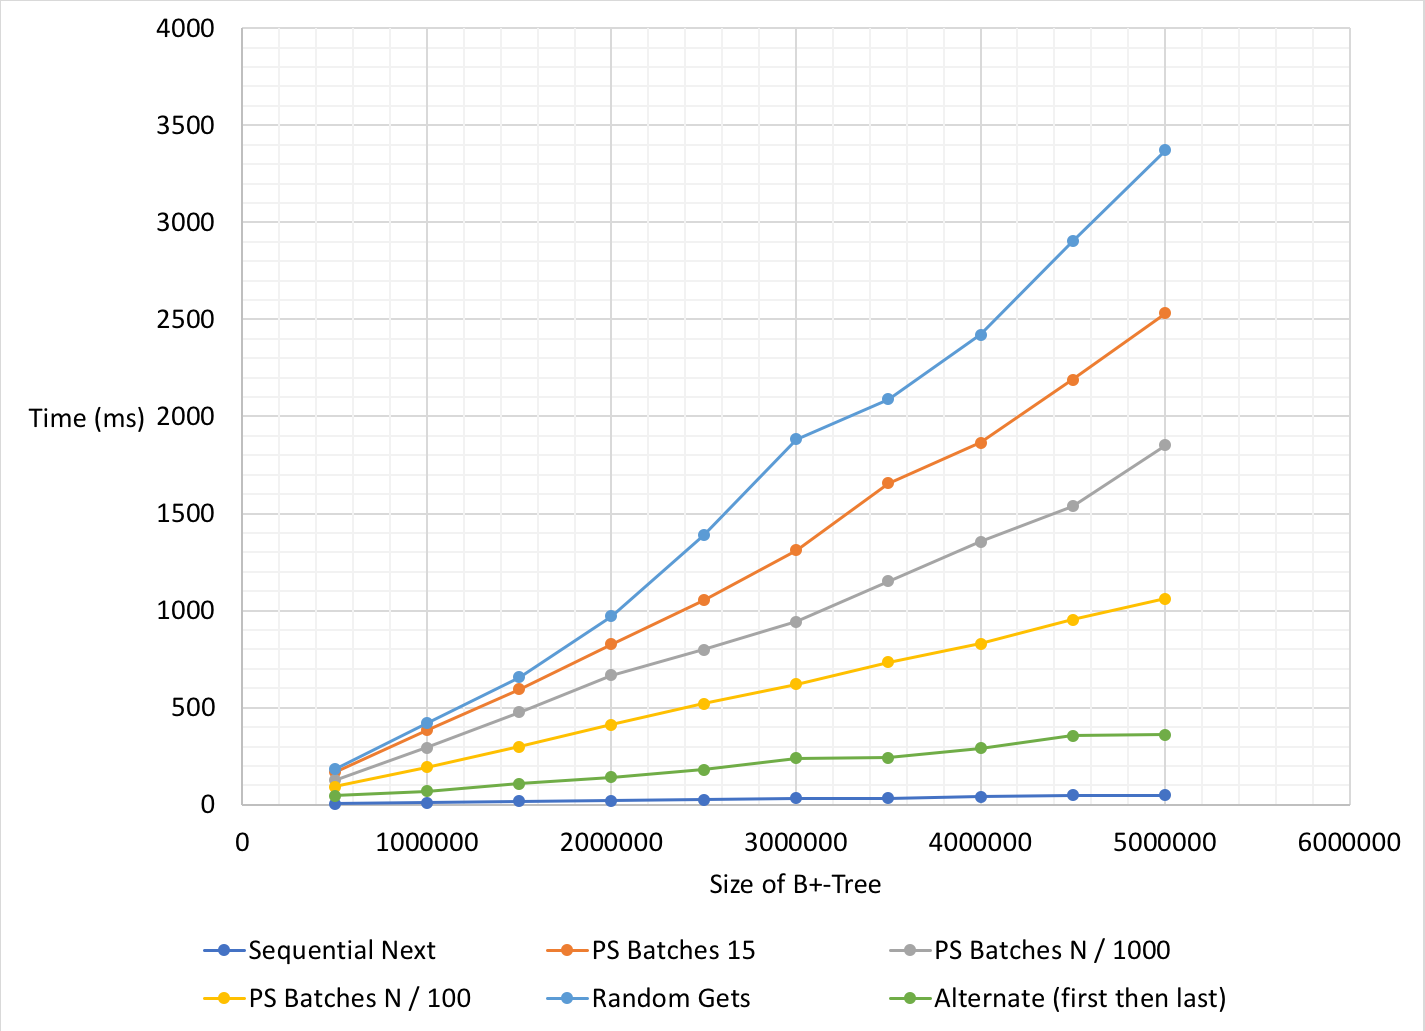
\includegraphics[scale=0.50]{figures/Btreegetsgraph.png}
    \caption{Time to visit or get all the keys in a B+-Tree for different B+-Tree sizes and different workloads.}
    \label{fig:B+GetsGraph}
\end{figure}

Similarly to evaluate the performance of B+-Tree put operations, we timed how long it took to insert a sequence of keys into the B+-Tree with the aforementioned workloads (sequential, partially-sorted and random). Results are shown in Figure \ref{fig:B+PutsGraph} Finally, we use the doubling hypothesis \cite{sedgewick2011algorithms} to empirically measure the order of growth of sequential and random operations . The doubling hypothesis states that if $T(N) \sim aN^blgN$ then $\frac{T(2N)}{T(N)} \sim 2^b$. So by calculating the log ratios of the times taken, we can estimate the order of growth of our B+-Tree under different workloads. 




\begin{figure}[htbp]
    \centering
    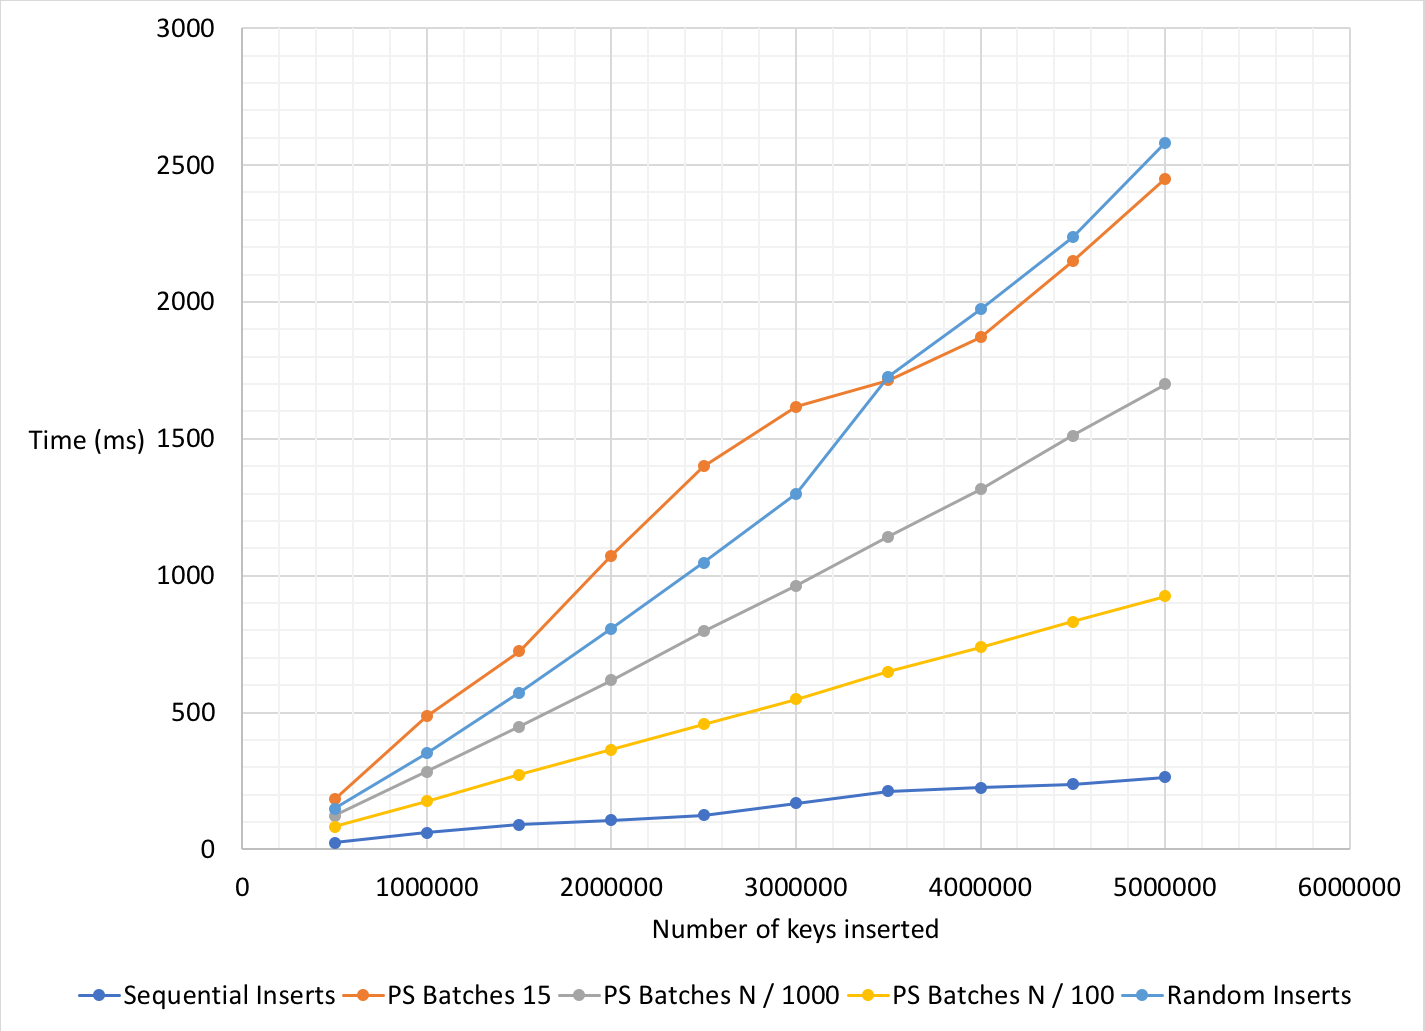
\includegraphics[scale=0.50]{figures/Btreeinsertsgraph.png}
    \caption{Time to insert all keys from 0 to size - 1 into an empty B+-Tree for different sizes and different workloads.}
    \label{fig:B+PutsGraph}
\end{figure}


As we can see from Figures \ref{fig:B+GetsGraph} and \ref{fig:B+PutsGraph} sequential operations are very fast inx our B+-Tree, while random operations are the slowest. We also see that our B+-Trees have performance gains if a series of put or get operations are partially sorted into sorted batches. The larger the sorted batches are in proportion to the number of keys to be inserted or retrieved, the larger the performance gain. On a different note, we expected that alternately retrieving the first and last keys in the B+-Tree its size number of times would model the worst case performance, as each retrieval costs $2 \times height$ node accesses. Even though this should, in theory, model the B+-Tree's worst case behavior it does not in practice, because of caching. If the same two keys are constantly retrieved, the same same ancestor nodes are traversed each time to get from one key to the other. These nodes will be in higher levels of cache memory thereby keeping the cost of node accesses to retrieve each key very low. This experiment highlights the value of cache-friendly data structures when implementing main-memory databases and also highlights how costly main-memory look-ups can be in comparison to cache look-ups.


\begin{figure}[htbp]
    \centering
    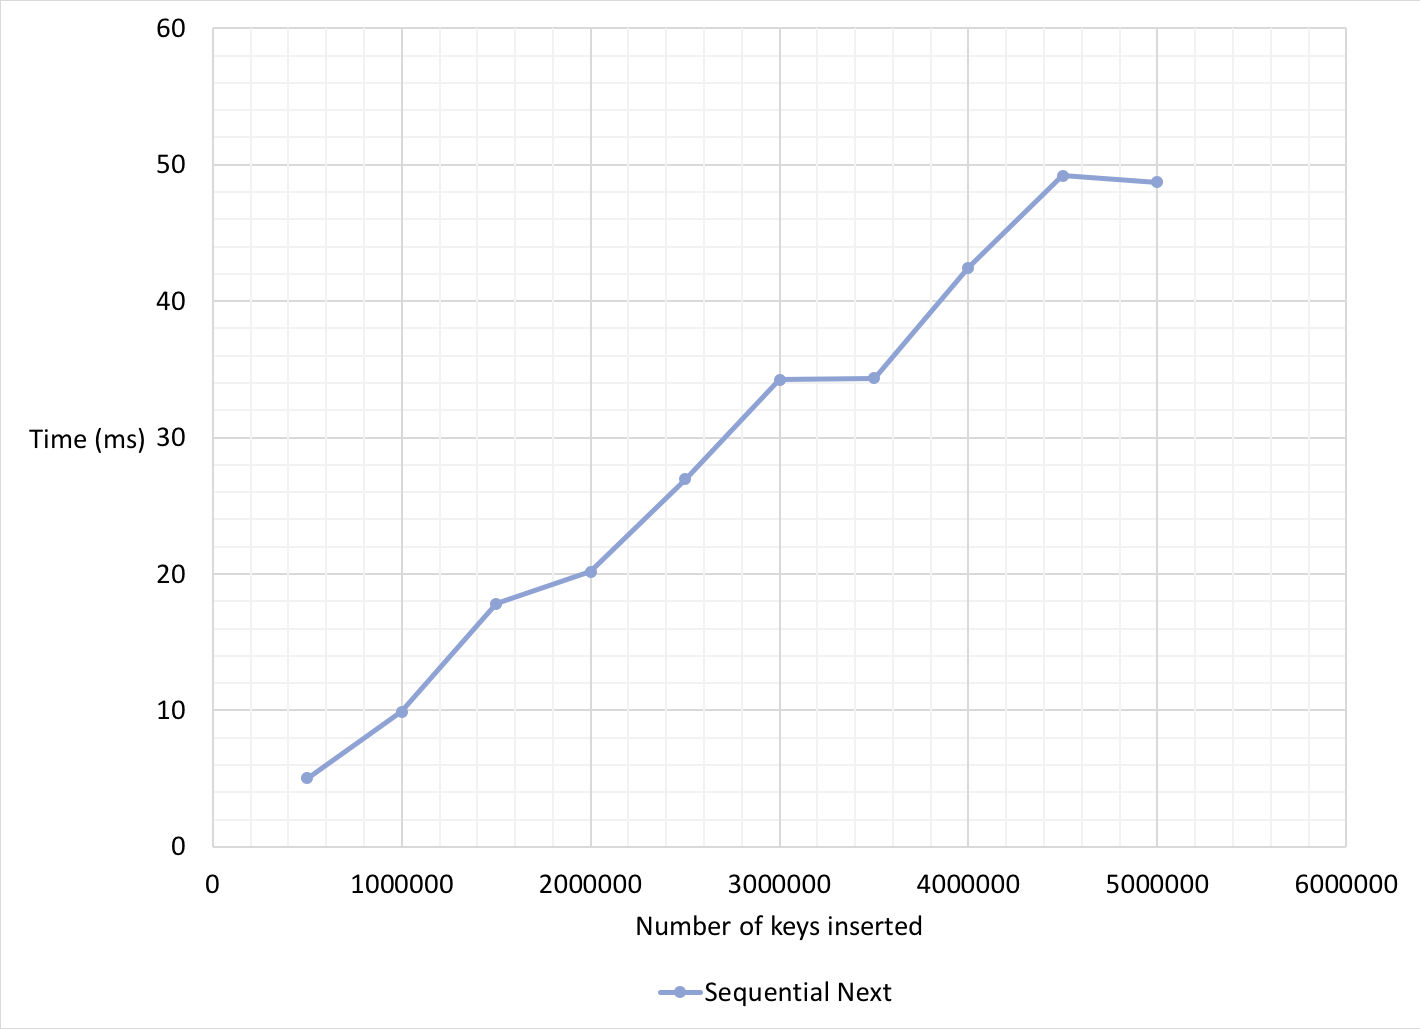
\includegraphics[scale=0.50]{figures/BtreeSequentialNextGraph.png}
    \caption{Time to sequentially visit all the keys in a B+-Tree for different B+-Tree sizes}
    \label{fig:B+GetsSequentialGraph}
\end{figure}

\begin{figure}[htbp]
    \centering
    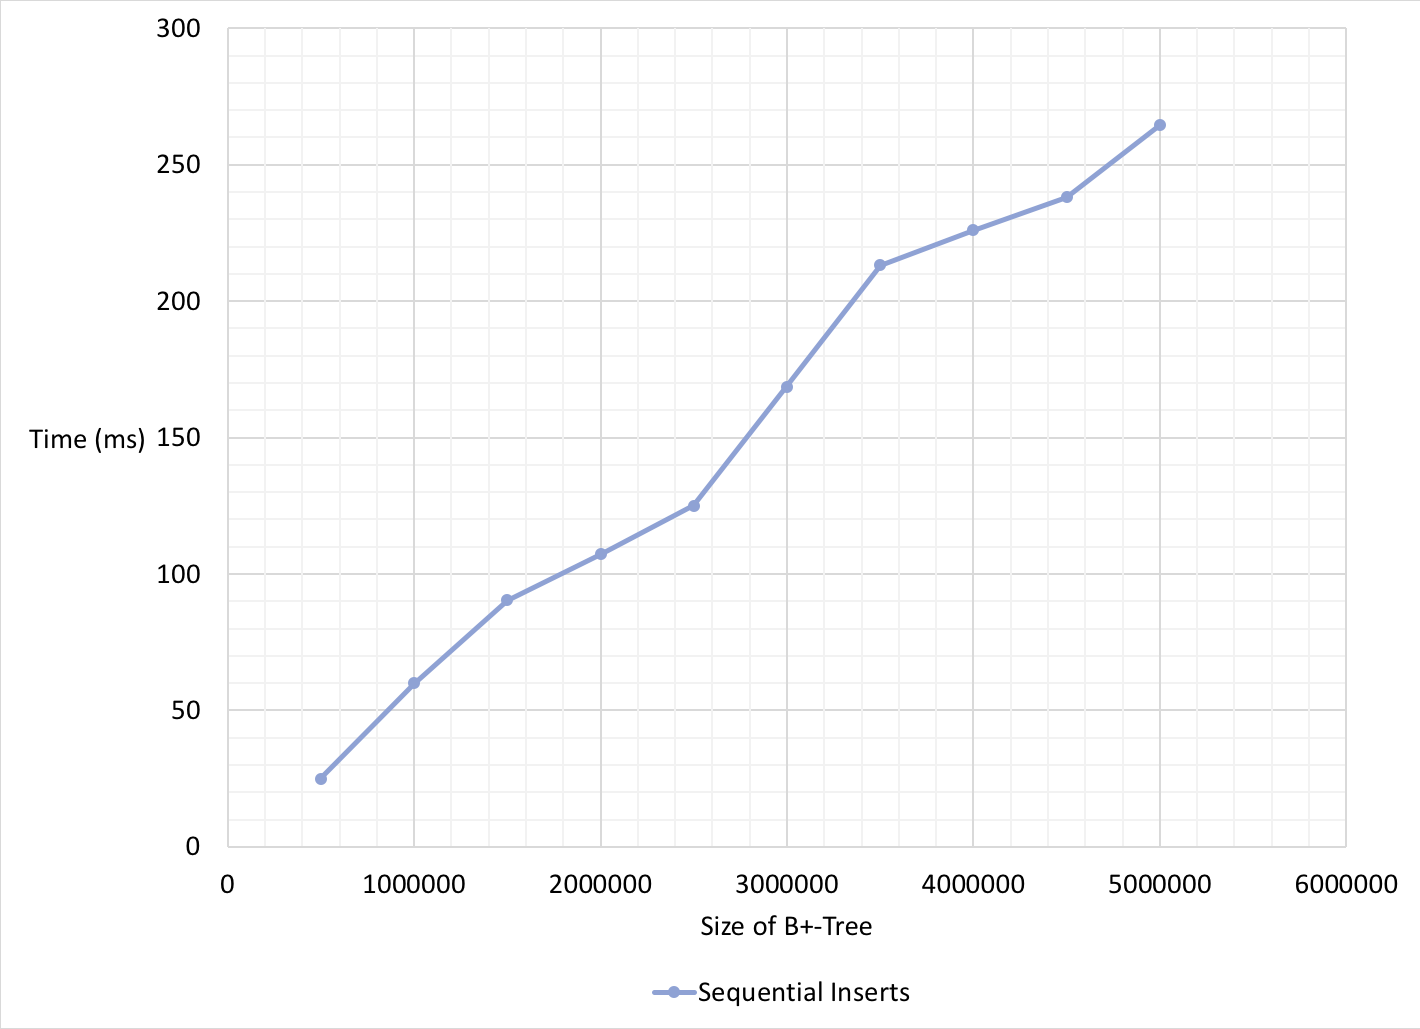
\includegraphics[scale=0.50]{figures/BtreeSequentialnsertsGraph.png}
    \caption{Time to sequentially insert all the keys from 0 to size - 1 into an empty B+-Tree}
    \label{fig:B+PutsSequentialGraph}
\end{figure}

Figures \ref{fig:B+GetsSequentialGraph} and \ref{fig:B+PutsSequentialGraph} allow us to better appreciate the speed of sequential operations. Our B+-Tree implementation can sequentially retrieve all keys from a B+-Tree of size 5 million in about 49 milliseconds; this is about 9.8 nanoseconds per next operation. We can sequentially insert 5 million keys into a B+-Tree in about 265 milliseconds; this is about 53 nanoseconds per next operation. 

\begin{table}[hbtp]
\centering
\label{fig:logRatioGetAnalysis}
\begin{tabular}{|c|c|c|c|c|}
\hline
\multirow{2}{*}{Number of keys (millions)} & \multicolumn{2}{c|}{Move to Next} & \multicolumn{2}{c|}{Random Get} \\ \cline{2-5} 
                                           & Time (ms)       & log ratio       & Time (ms)      & log ratio      \\ \hline
0.5                                        & 5.03            &                 & 182.48         &                \\ \hline
1                                          & 9.89            & 0.975           & 420.07         & 1.203          \\ \hline
2                                          & 20.16           & 1.027           & 970.84         & 1.209          \\ \hline
4                                          & 42.45           & 1.074           & 2421.73        & 1.319          \\ \hline
\end{tabular}
\caption{Log ratio of running times of sequential and random get operations for different key sizes.}
\end{table}

\begin{table}[htbp]
\centering
\label{fig:logRatioPutAnalysis}
\begin{tabular}{|c|c|c|c|c|}
\hline
\multirow{2}{*}{Number of keys (millions)} & \multicolumn{2}{c|}{Sequential Put} & \multicolumn{2}{c|}{Random Put} \\ \cline{2-5} 
                                           & Time (ms)       & log ratio       & Time (ms)      & log ratio      \\ \hline
0.5                                        & 25.01           &                 & 148.83         &                \\ \hline
1                                          & 59.89           & 1.260           & 350.62         & 1.236          \\ \hline
2                                          & 107.29          & 0.841           & 805.68         & 1.200          \\ \hline
4                                          & 225.94          & 1.074           & 1973.40        & 1.292          \\ \hline
\end{tabular}
\caption{Log ratio of running times of sequential and random put operations for different key sizes.}
\end{table}

Using the doubling hypothesis we see that the time complexity of $N$ sequential put or get operations is effectively linear (see see \ref{fig:logRatioGetAnalysis} and \ref{fig:logRatioPutAnalysis}). The log ratio converges to approximately one. However for random operations, even though the log ratio rounds down to 1, the fractional portion hints at an extra logarithmic term. This is in line with our expectation that $N$ random put or get operations is linearithmic.


\subsection{KVStore Experiments}

In this section we evaluate the following claims that our key-value store library: 
\begin{itemize}
    \item performs well when its keys have long common prefixes
    \item benefits from performance improvements when a sequence of operations is partially sorted by key.
\end{itemize}


\begin{figure}[h]
    \centering
    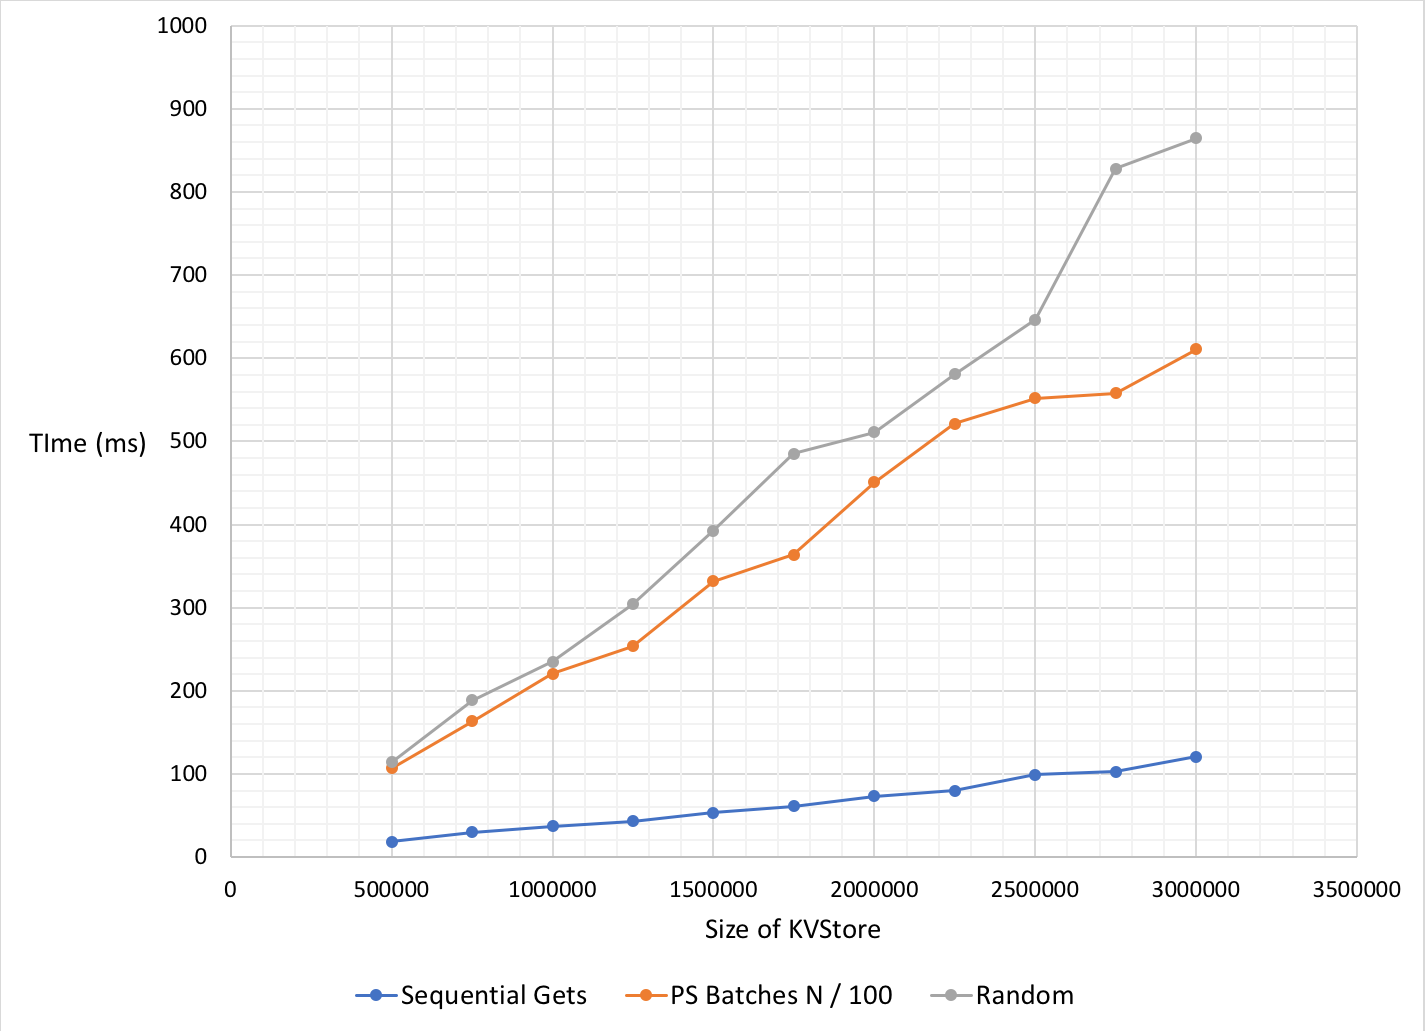
\includegraphics[scale=0.50]{figures/KVStoregetsgraph.png}
    \caption{Time to get all the keys in a KVStore for different sizes and different workloads. Keys are 30 bytes long and are not forced to have common prefixes. Keys are randomly generated.}
    \label{fig:KVStoreGetsGraph}
\end{figure}

Similarly to the B+-Tree experiments we evaluated how long it takes to retrieve all the keys in a KVStore object for different sizes and workloads, where each KVStore object is built with random keys. The results are in \ref{fig:KVStoreGetsGraph}. We see that, as expected sequential gets are very fast. We also see that partially sorting query keys gives performance gains over random query keys. However, the performance gains form partially sorting are not as large as one might expect. There could be different reasons for this. A possibility is that even if the next key being inserted or retrieved is different from the previous key on only the last few bytes, our current KVStore implementation still traverses the trie of B+-Trees from the first layer to the appropriate layer where the keys diverge. Even though we can skip all the layers where the key slices of the next key are the same as the previous key's key slices.


\begin{figure}[h]
    \centering
    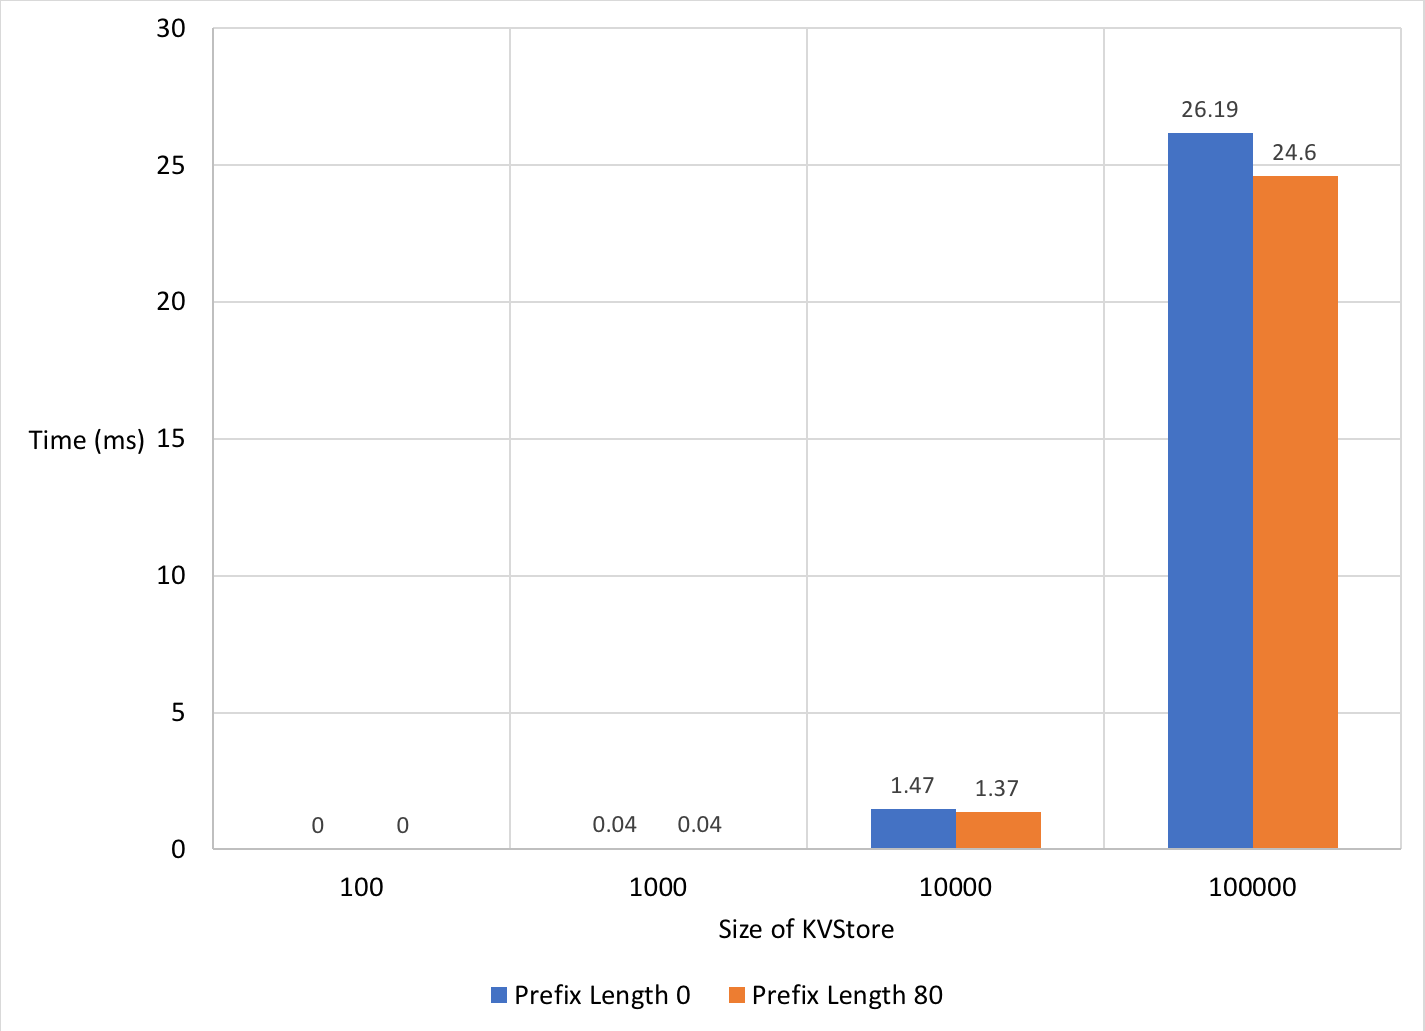
\includegraphics[scale=0.50]{figures/kvstoreprefixgraph.png}
    \caption{Time to get all the keys in a KVStore for different sizes for different common prefix lengths. Keys are 100 bytes long. We compare the behavior of get operations when the first 80 bytes are the same and the remaining 20 bytes are random versus when all 100 bytes are random. Keys are randomly generated.}
    \label{fig:KVStoreCommonPrefixes}
\end{figure}

From our discussion in section \ref{sec:VarLCPKeysMasstree}, the expectation is that a typical B+-Tree implementation and, by extension, a key-value store built from this B+-Tree would suffer performance degradation when most of its keys have long common prefixes. However, our KVStore implementation properly handles this scenario as shown in Figure \ref{fig:KVStoreCommonPrefixes}.In fact our KVStore does slightly better for keys with long common prefixes. This is probably because the first few layers of the KVStore consists of only two nodes each (a B+-Tree leaf node with one entry and a bordernode). Consequently, to get to any key all the nodes containing the common prefix must be visited and so these nodes will be in higher levels of cache memory.

\section{Future Work}

Our key-value store implementation is far from finished. There are a myriad of ways in which this key-value store can and should be improved upon. We will at least need to implement deletion for both the KVStore module and the B+-Tree module, among some other operations. It would also be good to add durability and support for concurrency. We would also like to extend the B+-Tree cursor concept to create and implement a KVStore Cursor (see Figure \ref{fig:KVStoreCursor1}). 

\begin{figure}[h]
    \centering
    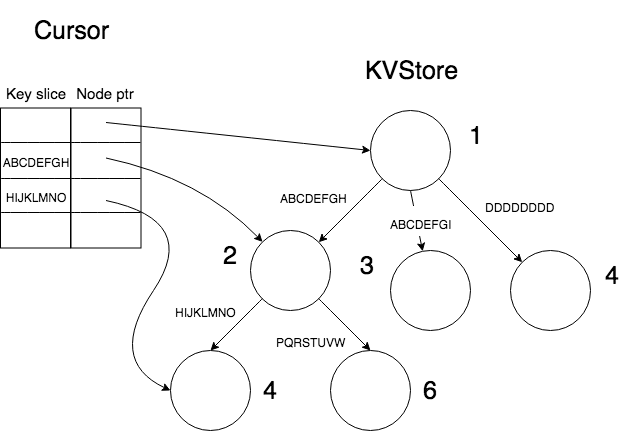
\includegraphics[scale=0.50]{figures/kvcursor1.png}
    \caption{KVStore Cursor at node 4.}
    \label{fig:KVStoreCursor1}
\end{figure}

\begin{figure}[h]
    \centering
    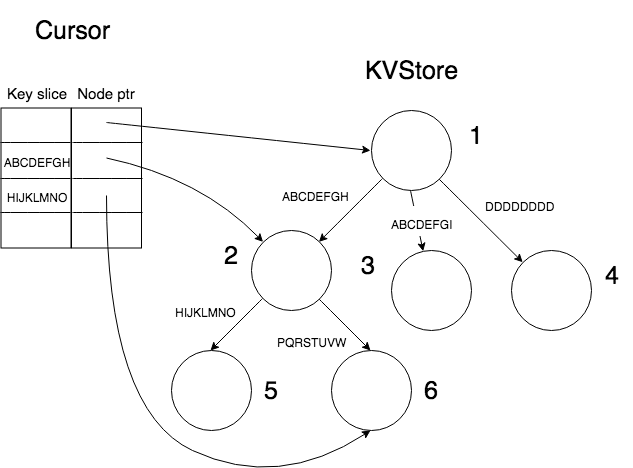
\includegraphics[scale=0.50]{figures/kvcursor2.png}
    \caption{KVStore Cursor at node 6.}
    \label{fig:KVStoreCursor2}
\end{figure}

The KVStore cursor is analogous to the B+-Tree cursor; ancestor nodes in the B+-Tree correspond to ancestor B+-Trees / layers in the KVStore. However, with a KVStore cursor, we would need to also store the key slice that each cursor is located at. This could drastically improve the cost of sequential inserts. This means that when the key of the next operation and the KVStore cursor's current key share a long common prefix, many layers in the KVStore data structure (the trie) will be skipped at the cost of only comparing the search key with the characters associated with each level of the KVStore cursor. We expect this cost to be significantly lower than traversing multiple layers of the overall tree data structure (which also involves navigating through each layer) to get to the desired key. However, it is important to note that if the search keys are totally random, there might be little or not benefit to this scheme. In fact, there would be the added overhead of maintaining KVStore cursor information. 

\begin{comment}
Interesting how in the past sequential i/o was crucial and now this cursor of cursors idea grants great gains when one operates on tree data structures sequentially. 
\end{comment}

\section{Conclusion}
In this Thesis Paper, we have described at a high-level the implementation of our main-memory serial key-value store. We gave a quick overview of main-memory databases, B+-Trees and Masstree in section \ref{sec:Background}. We discuss out key-value store implementation, B+-Tree with cursor implementation and why B+-Tree sequential operations take amortized constant time in section \ref{sec:Our System}. We also learn more about SQLite's \cite{SQLite} B+-Tree with cursor scheme and how it is used in our system. We evaluated the behaviour of our B+-Tree library and KVStore library in section \ref{sec:Evaluation}. Here we saw that the B+-Tree with cursor idea does indeed yield amortized constant time sequential\textbf{get} and \textbf{put} operations (traditional B+-Tree's can only guarantee constant time \textbf{get} operations). Moreover, we have shown that partially sorting a sequence of inputs leads to performance gains for our B+-Tree and KVStore. We have also shown that Masstree's trie of B+-Tree scheme can properly handle long common prefixes. Finally, we briefly presented a way to extend the B+-Tree cursor to a KVStore Cursor to further speed up sequential and partially sorted queries in our system. 

 

% Make the bibliography single spaced
\singlespacing
\bibliographystyle{plain}

% add the Bibliography to the Table of Contents
\cleardoublepage
\ifdefined\phantomsection
  \phantomsection  % makes hyperref recognize this section properly for pdf link
\else
\fi
\addcontentsline{toc}{section}{References}

% include your .bib file
\bibliography{thesis}

\end{document}

